\documentclass[
]{jss}

\usepackage[utf8]{inputenc}

\providecommand{\tightlist}{%
  \setlength{\itemsep}{0pt}\setlength{\parskip}{0pt}}

\author{
H. Sherry Zhang\\Monash University \And Dianne Cook\\Monash University
\AND Ursula Laa\\University of Natural Resources and Life Sciences
\AND Nicolas Langrené\\BNU-HKBU United International College
\AND Patricia Menéndez\\Monash University \AND
}
\title{\pkg{cubble}: An R Package for Structuring Spatio-temporal Data}

\Plainauthor{H. Sherry Zhang, Dianne Cook, Ursula Laa, Nicolas
Langrené, Patricia Menéndez}
\Plaintitle{cubble: An R Package for Structuring Spatio-temporal Data}

\Abstract{
Spatio-temporal variables can be time invariant or not and this divides
them into those can be identified only with the spatial identifier and
those cross-identified by the spatial and temporal identifier. In this
paper, a new data structure, \code{cubble}, is proposed for manipulating
and visualising spatio-temporal data. The new data structure proposes
two forms for manipulating the spatial and temporal dimension separately
while providing a smooth switch between the two forms to link the two
dimensions. Advanced considerations are given to illustrate data with
hierarchical structure, data matching, and how \pkg{cubble} fits with
interactive graphics pipeline. Examples are given to analysing Australia
meteorology data, river level data, and climate reanalysis (ERA5).
}

\Keywords{spatio temporal, \proglang{R}, climate weather station, data
analysis}
\Plainkeywords{spatio temporal, R, climate weather station, data
analysis}

%% publication information
%% \Volume{50}
%% \Issue{9}
%% \Month{June}
%% \Year{2012}
%% \Submitdate{}
%% \Acceptdate{2012-06-04}

\Address{
    H. Sherry Zhang\\
    Monash University\\
    21 Chancellors Walk, Clayton VIC 3800 Australia\\
  E-mail: \email{huize.zhang@monash.edu}\\
  
      Dianne Cook\\
    Monash University\\
    21 Chancellors Walk, Clayton VIC 3800 Australia\\
  E-mail: \href{mailto:dicook@monash.edu}{\nolinkurl{dicook@monash.edu}}\\
  
      Ursula Laa\\
    University of Natural Resources and Life Sciences\\
    Gregor-Mendel-Straße 33, 1180 Wien, Austria\\
  E-mail: \href{mailto:ursula.laa@boku.ac.at}{\nolinkurl{ursula.laa@boku.ac.at}}\\
  
      Nicolas Langrené\\
    BNU-HKBU United International College\\
    2000 Jintong Road, Tangjiawan, Zhuhai, Guangdong Province, China\\
  E-mail: \href{mailto:nicolas@langrene.com}{\nolinkurl{nicolas@langrene.com}}\\
  
      Patricia Menéndez\\
    Monash University\\
    21 Chancellors Walk, Clayton VIC 3800 Australia\\
  E-mail: \href{mailto:patricia.menendez@monash.edu}{\nolinkurl{patricia.menendez@monash.edu}}\\
  
  }

% Pandoc citation processing

% Pandoc header

\usepackage{amsmath} \usepackage{array} \usepackage{xcolor}

\begin{document}

\newpage

\hypertarget{introduction}{%
\section{Introduction}\label{introduction}}

Spatio-temporal data concerns variables in the spatial coordinates
across time. Some variables are invariant to time and can be solely
identified by its spatial location while other time varying variables
need both the spatial and temporal identifier to identify. Manipulating
data in these two levels is usually done separately and the third tidy
data principal \citep{tidydata} recommends each type of observational
unit to form a table. Another feature for a spatio-temporal data
structure to have is that variables created from subsequent operations
can be automatically added to the existing table with the same level.
This is better than an output that index the variables with the
identifiers since otherwise analysts will need to manually join this
output with existing variables in the same level.

Currently, available spatio-temporal data structure in R includes:
\pkg{spacetime} \citep{spacetime}, which proposes four space-time
layouts: Full grid (STF), sparse grid(STS), irregular (STI), and
trajectory (STT). The data structure it uses is based on \pkg{sp}
\citep{sp} and \pkg{xts} \citep{xts}, both of which has been replaced by
more recent implementations. \pkg{spatstat} \citep{spatstat} implements
a \texttt{ppp} class for point pattern data; and more recent,
\pkg{stars} \citep{stars} implements a spatio-temporal array with the
dplyr's data cube structure \pkg{cubelyr} \citep{cubelyr} as its
backend. While these implementations either store spatial and temporal
variables all in a single table, hence duplicate the spatial variables
for each temporal unit; or split them into two separate tables that has
the problem of manually joining, mentioned in the previously. This
creates a gap in the software development. The requirement for such a
tool is important given the ubiquity of spatio-temporal vector data in
the wild: the Ireland wind data from \pkg{gstat} is an classic example
data that splits variables into its spatial (\texttt{wind.loc}) and
temporal (\texttt{wind}) dimension; Bureau of Meteorology (BoM) provides
climate observations widely applied in agriculture and ecology study.

This paper describes the implementation of a new spatio-temporal data
structure: \pkg{cubble}. \pkg{cubble} implements a relational data
structure that uses two forms to manage the switch between spatial and
temporal dimension. With this structure, users can manipulate the
spatial or temporal dimension separately, while leaves the linking of
two dimensions to \pkg{cubble}. The software is available from the
Comprehensive R Archive Network (CRAN) at {[}CRAN link{]}.

The rest of the paper will be divided as follows: Section 2 presents the
workflow of data manipulation in cubble. Section 3 explains how cubble
deals with some advanced considerations including data with hierarchical
structure, data matching, and how cubble fits with existing static and
interactive visualisation tools. Section 4 gives examples of the
features introduced in the previous two sections with climate and
hydrology data. An example on how cubble handle Netcdf data is also
provided. Section 5 concludes the paper.

\hypertarget{the-cubble-package}{%
\section{The cubble package}\label{the-cubble-package}}

Spatio-temporal data usually come in various forms and Figure
\ref{fig:illu-input} shows four examples of this. No matter which form
the data is in, these formats share some common components that
characterise the spatio-temporal data. A spatial identifier (\code{id}
in the diagram) is the unique identifier of each site. The temporal
identifier (\code{t} in the diagram) prescribes the time stamp each site
is recorded. Coordinates, comprising of latitude and longitude
(\code{lat} and \code{(long)} in the diagram), locates each site on the
map. These identifiers will be the building blocks for the data
structure introduced below. Other variables in the data can be
categorised into two groups: spatial variables that are invariant at
each time stamp for every site, i.e.~the name or code of the weather
station, and temporal variables that varies with time.

\begin{CodeChunk}
\begin{figure}

{\centering 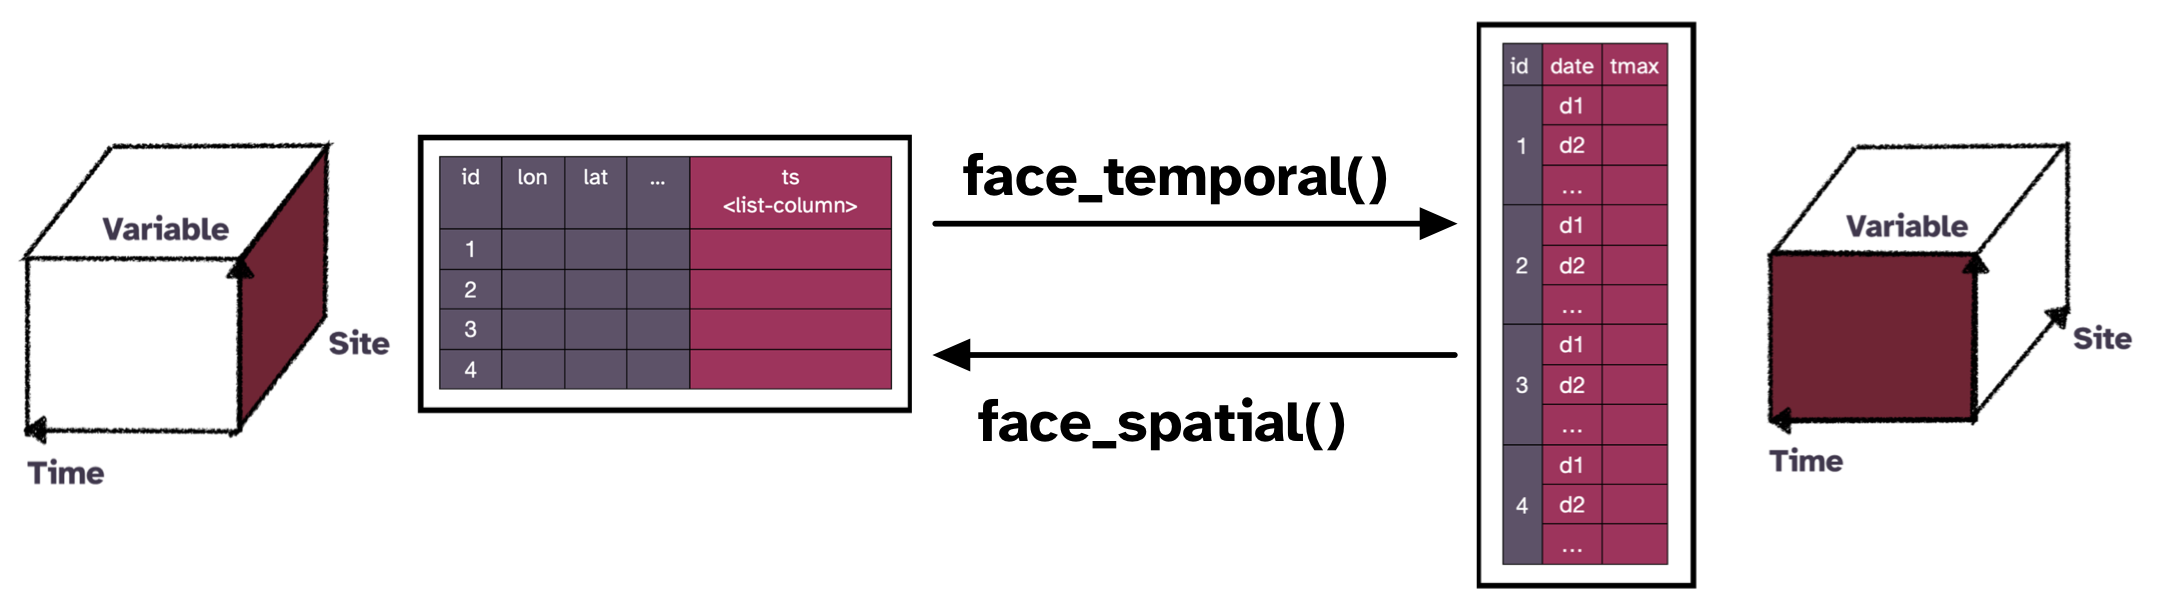
\includegraphics[width=1\linewidth,height=0.4\textheight]{/Users/sherryzhang/Documents/research/paper-cubble/figures/diagram-keynotes/diagram-keynotes.001} 

}

\caption[Illustration of incoming data formats for spatio-temporal data]{Illustration of incoming data formats for spatio-temporal data. (1) Data comes in as a single table; (2) Separate tables for spatial and temporal variables; (3) A single table with all the parameters used to query the database and a separate table for queried data; and (4) Cubical data in array or NetCDF format.}\label{fig:illu-input}
\end{figure}
\end{CodeChunk}

In a cubble, there are two forms: nested form and long form, and Figure
\ref{fig:illu-cubble} sketches the two forms along with the associated
attributes. The decision on which form to use is output-oriented,
meaning analysts need to first think about whether the output of a
particular operation is identified only by the spatial identifier, or a
combination of spatial and temporal identifier. The nested cubble is
suitable for working with operations that are only identified by the
site and this type of operation can be a pure manipulation of spatial
variables, or a summary of temporal variables by site (i.e.~the output
of counting the number of raining day is only identified by sites and
hence should be performed with the nested form). Underneath the nested
form, a cubble is built from a row-wise dataframe (\code{rowwise_df})
where each site forms a separate group. This structure simplifies the
calculation that involves temporal variables by avoiding the use of
\code{map} syntax when working with list-column.

For those operations whose output involves both a spatial and temporal
dimension, long form should be used. The long form is identified by both
the spatial and temporal identifier and adopts a grouped dataframe
(\texttt{grouped\_df}) to forms each site as a group. Spatial variables
are stored separately in a \pkg{tibble} as an special attribute of the
long cubble. This design avoids repeating the spatial variables at each
time stamp while not dropping information from spatial variables.

\begin{CodeChunk}
\begin{figure}

{\centering 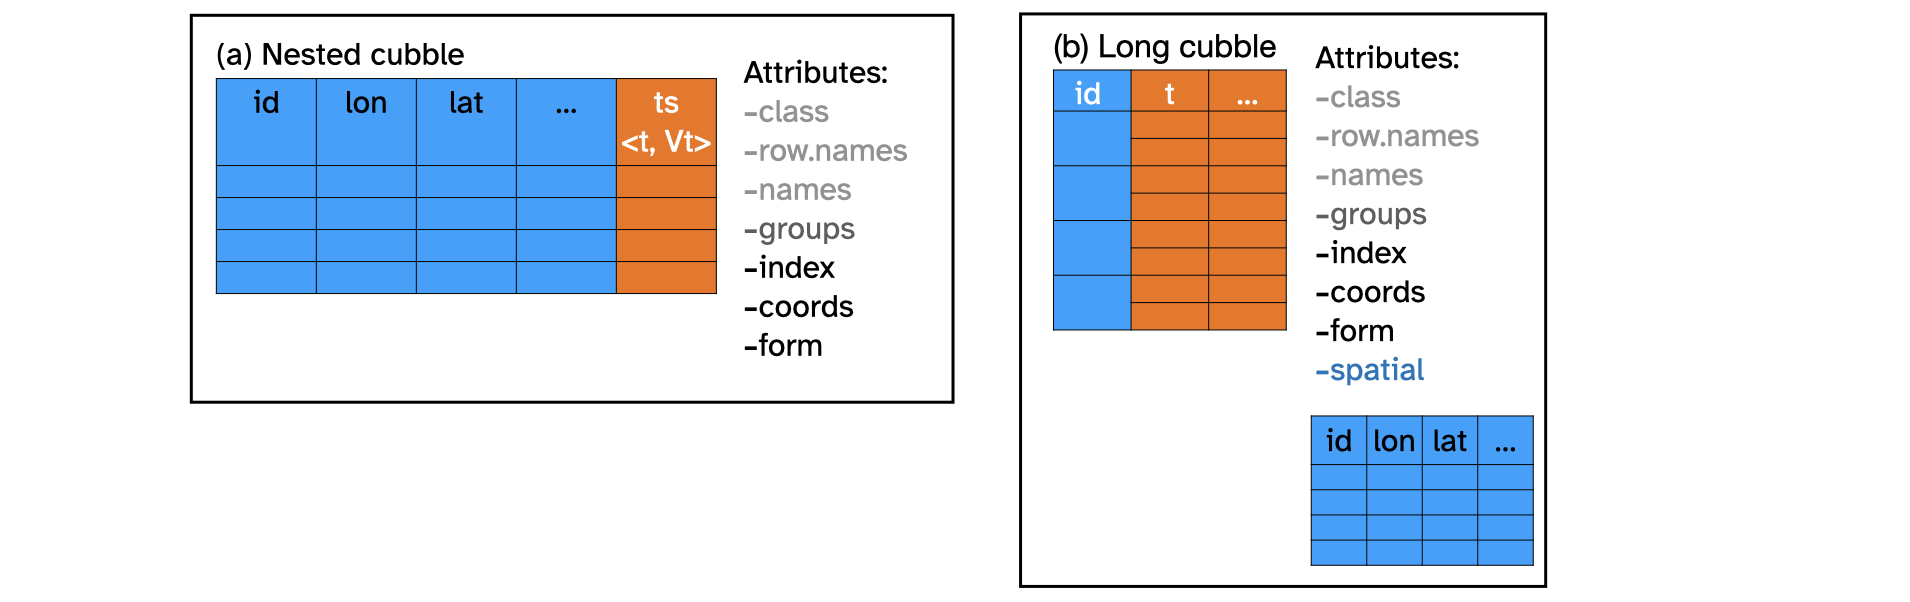
\includegraphics[width=1\linewidth]{/Users/sherryzhang/Documents/research/paper-cubble/figures/diagram-keynotes/diagram-keynotes.002} 

}

\caption[Illustration of nested and long cubble]{Illustration of nested and long cubble.}\label{fig:illu-cubble}
\end{figure}
\end{CodeChunk}

\hypertarget{create-a-cubble-in-the-nested-form}{%
\subsection{Create a cubble in the nested
form}\label{create-a-cubble-in-the-nested-form}}

`as\_cubble()\} creates a \pkg{cubble} by supplying the three key
components: \code{key} as the spatial identifier; \code{index} as the
temporal identifier; and a vector of \code{coords} in the order of
longitude first and then latitude. The naming of \code{key} and
\code{index} follows the convention in the \pkg{tsibble} package. The
cubble created by default is in the nested form. Below is an example of
creating a cubble:

\begin{CodeChunk}
\begin{CodeInput}
R> cubble_nested <- cubble::climate_flat %>%
+   as_cubble(key = id, index = date, coords = c(long, lat))
R> cubble_nested
\end{CodeInput}
\begin{CodeOutput}
# cubble:   id [5]: nested form
# bbox:     [115.97, -32.94, 133.55, -12.42]- check gap on long and lat
# temporal: date [date], prcp [dbl], tmax [dbl], tmin [dbl]
  id            lat  long  elev name           wmo_id ts                
  <chr>       <dbl> <dbl> <dbl> <chr>           <dbl> <list>            
1 ASN00009021 -31.9  116.  15.4 perth airport   94610 <tibble [366 x 4]>
2 ASN00010311 -31.9  117. 179   york            94623 <tibble [366 x 4]>
3 ASN00010614 -32.9  117. 338   narrogin        94627 <tibble [366 x 4]>
4 ASN00014015 -12.4  131.  30.4 darwin airport  94120 <tibble [366 x 4]>
5 ASN00015131 -17.6  134. 220   elliott         94236 <tibble [366 x 4]>
\end{CodeOutput}
\end{CodeChunk}

There are a few information in the \pkg{cubble} header: the name of the
\code{key} variable (\texttt{id}) and its number (5), bounding box
(\texttt{{[}115.97,\ -32.94,\ 133.55,\ -12.42{]}}), and also the name of
variable nested in the \code{ts} column with its type:
\code{date [date], prcp [dbl], tmax [dbl], tmin [dbl]}.

\hypertarget{stretch-a-nested-cubble-into-the-long-form}{%
\subsection{Stretch a nested cubble into the long
form}\label{stretch-a-nested-cubble-into-the-long-form}}

The long cubble is suitable to manipulate the time dimension of the
data. The function \code{stretch()} switches the nested cubble into the
long cubble by first extracts all the spatial variables into a separate
tibble and store in the \code{spatial} attribute and then unnests the
\code{ts} column:

\begin{CodeChunk}
\begin{CodeInput}
R> cubble_long <- cubble_nested %>% stretch(ts)
R> cubble_long
\end{CodeInput}
\begin{CodeOutput}
# cubble:  date, id [5]: long form
# bbox:    [115.97, -32.94, 133.55, -12.42]- check gap on long and lat
# spatial: lat [dbl], long [dbl], elev [dbl], name [chr], wmo_id [dbl]
  id          date        prcp  tmax  tmin
  <chr>       <date>     <dbl> <dbl> <dbl>
1 ASN00009021 2020-01-01     0  31.9  15.3
2 ASN00009021 2020-01-02     0  24.9  16.4
3 ASN00009021 2020-01-03     6  23.2  13  
4 ASN00009021 2020-01-04     0  28.4  12.4
5 ASN00009021 2020-01-05     0  35.3  11.6
# ... with 1,825 more rows
\end{CodeOutput}
\end{CodeChunk}

Notice here that the third line in the header now shows the name and
type of spatial variables:
\code{lat [dbl], long [dbl], elev [dbl], name [chr], wmo_id [dbl]}.

\hypertarget{tamp-a-long-cubble-back-to-the-nested-form}{%
\subsection{Tamp a long cubble back to the nested
form}\label{tamp-a-long-cubble-back-to-the-nested-form}}

Manipulation on the spatial and temporal dimension can be an iterative
process. Many times, analysts will need to go back and forth between the
nested and long cubble. \code{tamp()} inverses the \code{stretch()} that
introduced in the previous section, to switch from a long cubble to the
nested cubble:

\begin{CodeChunk}
\begin{CodeInput}
R> cubble_back <- cubble_long %>% tamp()
R> cubble_back
\end{CodeInput}
\begin{CodeOutput}
# cubble:   id [5]: nested form
# bbox:     [115.97, -32.94, 133.55, -12.42]- check gap on long and lat
# temporal: date [date], prcp [dbl], tmax [dbl], tmin [dbl]
  id            lat  long  elev name           wmo_id ts                
  <chr>       <dbl> <dbl> <dbl> <chr>           <dbl> <list>            
1 ASN00009021 -31.9  116.  15.4 perth airport   94610 <tibble [366 x 4]>
2 ASN00010311 -31.9  117. 179   york            94623 <tibble [366 x 4]>
3 ASN00010614 -32.9  117. 338   narrogin        94627 <tibble [366 x 4]>
4 ASN00014015 -12.4  131.  30.4 darwin airport  94120 <tibble [366 x 4]>
5 ASN00015131 -17.6  134. 220   elliott         94236 <tibble [366 x 4]>
\end{CodeOutput}
\end{CodeChunk}

\hypertarget{migrate-spatial-variables-to-a-long-cubble}{%
\subsection{Migrate spatial variables to a long
cubble}\label{migrate-spatial-variables-to-a-long-cubble}}

Some functions require time invariant variables to be in the same table
as the time varying ones. In cubble, this can be done through
\code{migrate()}, which moves the time invariant variables into the long
cubble:

\begin{CodeChunk}
\begin{CodeInput}
R> cubble_mig <- cubble_long %>% migrate(long, lat)
R> cubble_mig
\end{CodeInput}
\begin{CodeOutput}
# cubble:  date, id [5]: long form
# bbox:    [115.97, -32.94, 133.55, -12.42]- check gap on long and lat
# spatial: lat [dbl], long [dbl], elev [dbl], name [chr], wmo_id [dbl]
  id          date        prcp  tmax  tmin  long   lat
  <chr>       <date>     <dbl> <dbl> <dbl> <dbl> <dbl>
1 ASN00009021 2020-01-01     0  31.9  15.3  116. -31.9
2 ASN00009021 2020-01-02     0  24.9  16.4  116. -31.9
3 ASN00009021 2020-01-03     6  23.2  13    116. -31.9
4 ASN00009021 2020-01-04     0  28.4  12.4  116. -31.9
5 ASN00009021 2020-01-05     0  35.3  11.6  116. -31.9
# ... with 1,825 more rows
\end{CodeOutput}
\end{CodeChunk}

Notice that these added time invariant variables will not be remembered
the cubble and will disappear if switched to the nested form and then
switched back. Hence they should most likely been used at the last step
of the analysis:

\begin{CodeChunk}
\begin{CodeInput}
R> cubble_mig %>% tamp() %>% stretch()
\end{CodeInput}
\begin{CodeOutput}
# cubble:  date, id [5]: long form
# bbox:    [115.97, -32.94, 133.55, -12.42]- check gap on long and lat
# spatial: long [dbl], lat [dbl], elev [dbl], name [chr], wmo_id [dbl]
  id          date        prcp  tmax  tmin
  <chr>       <date>     <dbl> <dbl> <dbl>
1 ASN00009021 2020-01-01     0  31.9  15.3
2 ASN00009021 2020-01-02     0  24.9  16.4
3 ASN00009021 2020-01-03     6  23.2  13  
4 ASN00009021 2020-01-04     0  28.4  12.4
5 ASN00009021 2020-01-05     0  35.3  11.6
# ... with 1,825 more rows
\end{CodeOutput}
\end{CodeChunk}

\hypertarget{compatibility-with-existing-packages}{%
\subsection{Compatibility with existing
packages}\label{compatibility-with-existing-packages}}

Building from an \code{tbl_df} class, \pkg{cubble} has implemented
methods for \pkg{dplyr} generics, which includes:

\begin{itemize}
\tightlist
\item
  basic: mutate, filter, summarise, select, arrange, rename, left\_join
\item
  grouping: group\_by, ungroup
\item
  slice family: slice\_head, slice\_tail, slice\_sample, slice\_min,
  slice\_max
\end{itemize}

\pkg{cubble} is also compatible with \pkg{tsibble}. When creating a
cubble from a tsibble, Only the \code{coords} argument need to be
specified:

\begin{CodeChunk}
\begin{CodeInput}
R> # casting a tsibble into cubble
R> dt <- climate_flat %>% 
+   tsibble::as_tsibble(key = id, index = date) %>% 
+   cubble::as_cubble(coords = c(long, lat))
R> dt
\end{CodeInput}
\begin{CodeOutput}
# cubble:   id [5]: nested form
# bbox:     [115.97, -32.94, 133.55, -12.42]- check gap on long and lat
# temporal: date [date], prcp [dbl], tmax [dbl], tmin [dbl]
  id            lat  long  elev name           wmo_id ts                
  <chr>       <dbl> <dbl> <dbl> <chr>           <dbl> <list>            
1 ASN00009021 -31.9  116.  15.4 perth airport   94610 <tbl_ts [366 x 4]>
2 ASN00010311 -31.9  117. 179   york            94623 <tbl_ts [366 x 4]>
3 ASN00010614 -32.9  117. 338   narrogin        94627 <tbl_ts [366 x 4]>
4 ASN00014015 -12.4  131.  30.4 darwin airport  94120 <tbl_ts [366 x 4]>
5 ASN00015131 -17.6  134. 220   elliott         94236 <tbl_ts [366 x 4]>
\end{CodeOutput}
\end{CodeChunk}

In the created nested form, each element of the list-column \code{ts} is
of \code{tbl_ts} class so that existing operations on the tsibble class
can still be applied:

\begin{CodeChunk}
\begin{CodeInput}
R> # add station-based features in the nested form.
R> dt %>% 
+   mutate(fabletools::features(ts, tmax, list(tmax_mean = mean, tmax_var = var)))
\end{CodeInput}
\begin{CodeOutput}
# cubble:   id [5]: nested form
# bbox:     [115.97, -32.94, 133.55, -12.42]- check gap on long and lat
# temporal: date [date], prcp [dbl], tmax [dbl], tmin [dbl]
  id            lat  long  elev name           wmo_id ts      tmax_mean tmax_var
  <chr>       <dbl> <dbl> <dbl> <chr>           <dbl> <list>      <dbl>    <dbl>
1 ASN00009021 -31.9  116.  15.4 perth airport   94610 <tbl_t~      25.7    38.6 
2 ASN00010311 -31.9  117. 179   york            94623 <tbl_t~      26.2    51.1 
3 ASN00010614 -32.9  117. 338   narrogin        94627 <tbl_t~      23.7    45.4 
4 ASN00014015 -12.4  131.  30.4 darwin airport  94120 <tbl_t~      33.1     3.02
5 ASN00015131 -17.6  134. 220   elliott         94236 <tbl_t~      34.6    24.7 
\end{CodeOutput}
\end{CodeChunk}

\hypertarget{advanced-features-considerations}{%
\section{Advanced features/
considerations}\label{advanced-features-considerations}}

\hypertarget{hierarchical-structure}{%
\subsection{Hierarchical structure}\label{hierarchical-structure}}

Spatial locations can have grouping structure that is either inherent to
the data (i.e.~countries are nested in continents), or formed by
clustering. Rather than analysing variables in the site level,
summarised variables in the cluster level can give a crisper picture of
local areas. In cubble, \code{switch_key()} can be used to create a new
level of grouping of spatial location by specifying a clustering
variable. Figure \ref{fig:illu-hier} illustrates the relationship of
cubbles at station and cluster level, in both the long and nested form.
By specifying
\code{cluster_nested <- station_nested \%>\% switch_key(key = cluster)},
the cubble re-defines the cubble key from \code{id} in
\code{station_nested} to \code{cluster} in \code{cluster_nested}. All
the spatial variables variant to \code{cluster} are now nested into a
\code{.val} column and cluster level variables can be computed in the
same fashion as station level variables in \code{station_nested}.
Following the same principal of \code{stretch}. the long form cluster
level cubble expands the time series variables with both indices:
\code{cluster} and \code{id}. All the cluster level variables are stored
separately for recovering the nested from from the long form.

\begin{CodeChunk}
\begin{figure}

{\centering 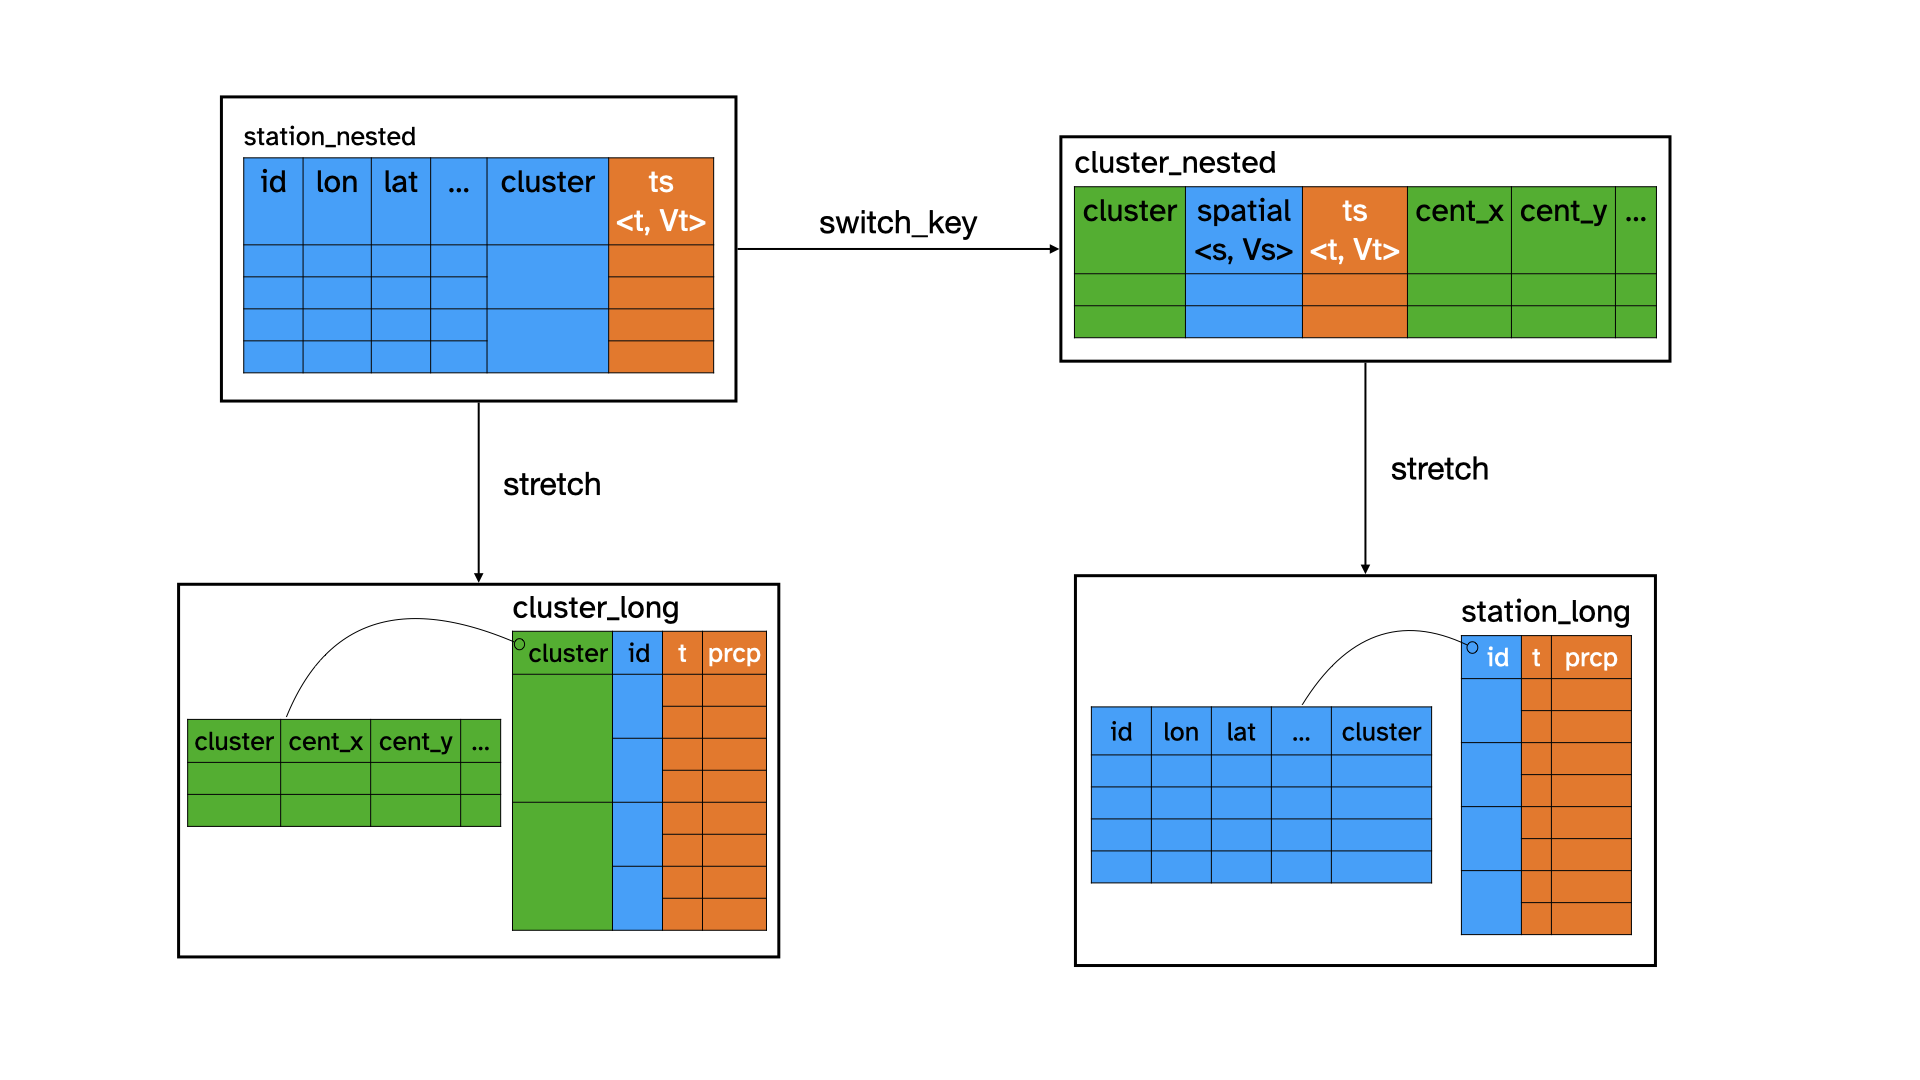
\includegraphics[width=1\linewidth,height=0.4\textheight]{/Users/sherryzhang/Documents/research/paper-cubble/figures/diagram-keynotes/diagram-keynotes.003} 

}

\caption[Relationship between the station and cluster level cubble in both long and nested form]{Relationship between the station and cluster level cubble in both long and nested form.}\label{fig:illu-hier}
\end{figure}
\end{CodeChunk}

\hypertarget{data-fusion-and-matching}{%
\subsection{Data fusion and matching}\label{data-fusion-and-matching}}

\textcolor{red}{refine the beginning.} To be a valid pair of matching,
the matched pair from different data sources need to

\begin{itemize}
\tightlist
\item
  be spatially close to each other, and
\item
  have similar temporal movement
\end{itemize}

`match\_sites()\} from \pkg{cubble} matches data based on these two
criteria. It first matches the two data sources spatially through
computing the pairwise distance based on latitude and longitude. Pairs
that pass the spatial matching are then matched temporally through
computing the number of matched peaks within a fixed length window.
Figure \ref{fig:illu-matching} illustrate this temporal matching in more
details. Given two series \code{A} and \code{a}. 3 peaks have been
picked in each series. An interval, with default length of 5, is
constructed for each peak in series \code{A} and the peaks in series
\code{a} are tested against whether they fall into the any of the
intervals. In this illustration, there are 2 matches for these two
series. Several arguments are available in \code{match_sites()} to
fine-tune the matching:

\begin{CodeChunk}
\begin{figure}

{\centering 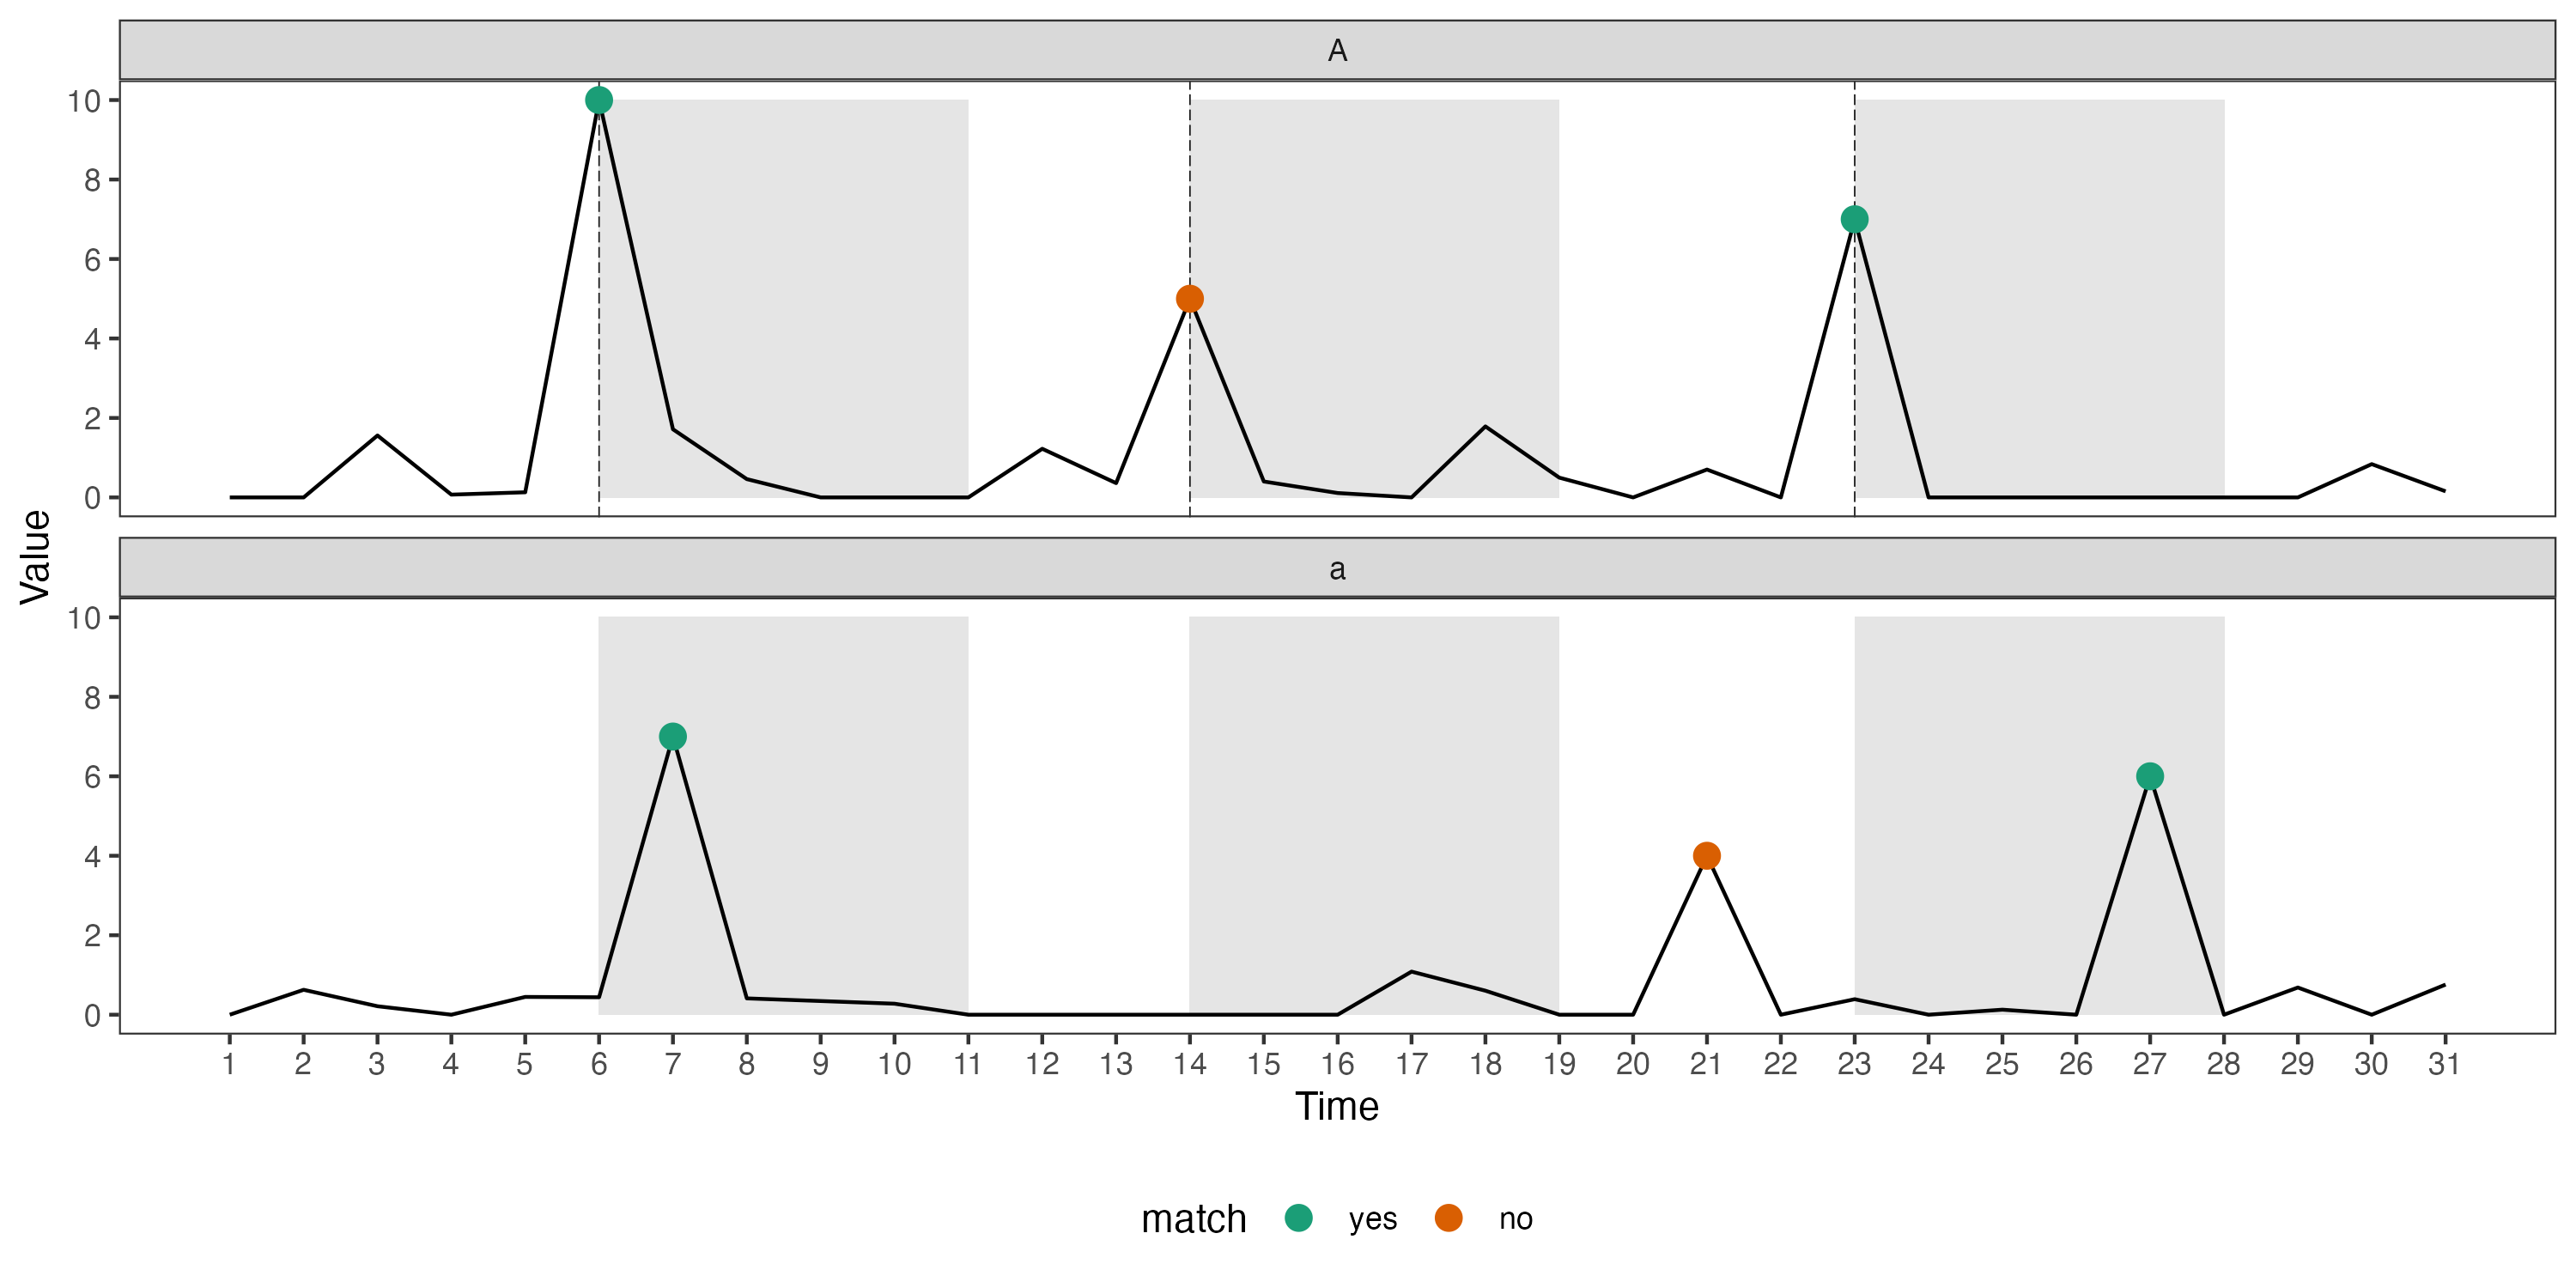
\includegraphics[width=1\linewidth]{figures/illu-matching} 

}

\caption[An illustration of temporal matching in cubble]{An illustration of temporal matching in cubble. Three highest peaks are identified in each series and intervals are constructed on series A. Two peaks in series a fall into the intervals and hence the two series are considered to have 2 matches.}\label{fig:illu-matching}
\end{figure}
\end{CodeChunk}

\begin{itemize}
\tightlist
\item
  \code{spatial_n_keep}. the number of spatial match for each site to
  keep
\item
  \code{spatial_dist_max}. the maximum distance allowed for a matched
  pair
\item
  \code{temporal_n_highest}. the number of peak used - 3 in the example
  above
\item
  \code{temporal_window}. the length of the interval - 5 in the example
  above
\item
  \code{temporal_min_match}. the minimum number of matched peak for a
  valid matched pair
\end{itemize}

This functionality can be seen as a matching
\citep{stuart2010matching, mcintosh2018using} exercise in the
spatio-temporal domain to pair up nearby observatoins. It can also be
considered as a form of data fusion
\citep{castanedo2013review, cocchi2019data}, where data from multiple
sources are combined together.

\hypertarget{interactive-graphics}{%
\subsection{Interactive graphics}\label{interactive-graphics}}

Cubble fits in naturally with the interactive graphic pipeline discussed
in the literature
\citep{buja1988elements, buja1996interactive, sutherland2000orca, xie2014reactive, cheng2016enabling}.
Diagram \ref{fig:illu-interactive} illustrates how linking works from
the map to the time series with the two forms of a cubble. The map and
time series plot is associated with the nested or long cubble
respectively and when a user action is captured on the map, the site
will be activated in the nested cubble (left). The nested cubble will
communicate to the long cubble to activate all the observations with the
same \code{id} (middle). The long cubble will then highlight the
activated series in the time series plot (right).

The linking is also available from the time series plot to the map. The
selection(s) on the time series is through selecting the point(s) on the
time series and once a point is selected, it will be activated in the
long cubble. All the observations that share the same \code{id} are then
activated and this includes other points in the same time series in the
long cubble and the corresponding observation of site in the nested
cubble. These activated observations will then being reflected in the
updated plots and Diagram \ref{fig:illu-interactive-2} in the Appendix
illustrates this process.

\begin{CodeChunk}
\begin{figure}

{\centering 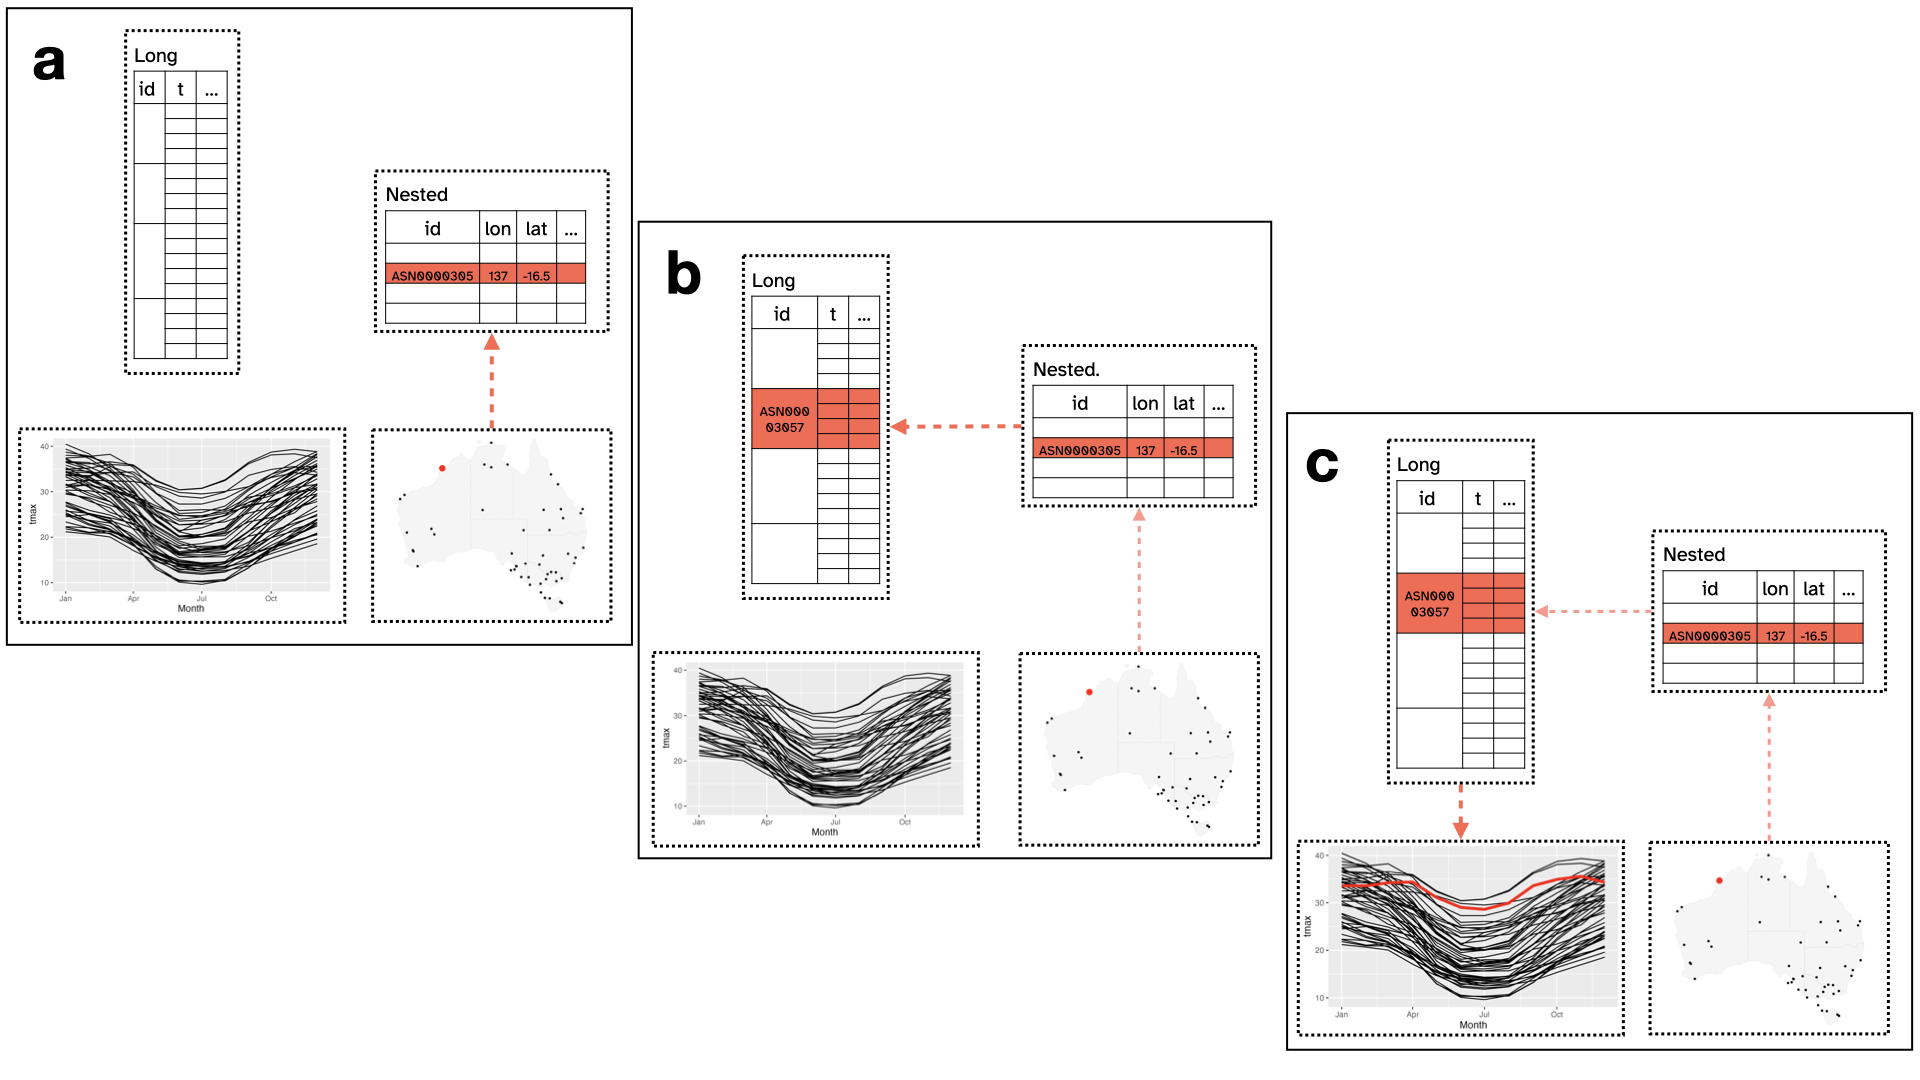
\includegraphics[width=1\linewidth,height=0.4\textheight]{/Users/sherryzhang/Documents/research/paper-cubble/figures/diagram-keynotes/diagram-keynotes.004} 

}

\caption[An illustration of the data model under interactive graphics with cubble]{An illustration of the data model under interactive graphics with cubble. The line plot and map is made separately with the long and nested cubble. When a station is selected on the map (left), the corresponding row in the nested cubble will be activated. This will link to all the rows with the same id in the long cubble (middle) and update the line plot (right).}\label{fig:illu-interactive}
\end{figure}
\end{CodeChunk}

\hypertarget{glyph-map}{%
\subsection{Glyph map}\label{glyph-map}}

Glyph map \citep{Wickham2012-yr} plots the time series as single glyph
on the map and in \proglang{R}, \pkg{GGally} implements the glyph map
through the \code{glyphs()} function. The function construct a data
frame with calculated position (`gx\}. \code{gy}. \code{gid}. of each
point on the time series using linear algebra (Equation 1 and 2 in
\citet{Wickham2012-yr}). The data can then be piped into \code{ggplot}
to create the glyph map as:

\begin{CodeChunk}
\begin{CodeInput}
R> library(ggplot2)
R> gly <- glyphs(data, 
+               x_major = ..., x_minor = ..., 
+               y_major = ..., y_minor = ..., ...)
R> 
R> ggplot(gly, aes(gx, gy, group = gid)) + 
+   geom_path() 
\end{CodeInput}
\end{CodeChunk}

A re-implementation of the glyph map as a ggproto \code{GeomGlyph} has
been made in the \pkg{cubble} package so that the glyph map can be
created with \code{geom_glyph()}:

\begin{CodeChunk}
\begin{CodeInput}
R> ggplot(data = data) +
+   geom_glyph(aes(x_major = ..., x_minor = ..., 
+                  y_major = ..., y_minor = ...))
\end{CodeInput}
\end{CodeChunk}

Polar glyph map can be specify as a parameter, \code{polar = TRUE}. in
the \code{geom_glyph()}. along with \code{width} and \code{height} in
either absolute or relative value. Global and local scale can be
controlled by the parameter \code{global_rescale}. which default to
\code{TRUE} for global scaling. Reference box and line can be added with
separate \code{geom_glyph_box()} and
\textbackslash code\{geom\_glyph\_line()`.

\hypertarget{examples}{%
\section{Examples}\label{examples}}

\hypertarget{australia-historical-maximum-temperature}{%
\subsection{Australia historical maximum
temperature}\label{australia-historical-maximum-temperature}}

Global Historical Climatology Network (GHCN) provides daily climate
measures from stations across the world and the dataset
\code{weatherdata::historical_tmax} extracts the maximum temperature for
236 Australian stations. All the stations start recording from year 1969
with the longest back to year 1859. The data \code{historical_tmax} is
already presented as a cubble, with \code{id} as the key, \code{date} as
the index, and \code{c(longitude, latitude)} as the coordinates. This
example compares the maximum temperature in two periods: 1971 - 1975 and
2016 - 2020 for stations in Victoria and New South Wales.

Stations in the two states can be subsetted by the station number:
Australia GHCN station number starts with ``ASN00'' and followed by the
\href{http://www.bom.gov.au/climate/cdo/about/site-num.shtml}{Bureau of
Meteorology (BOM) station number}, where the 2nd and 3rd digit (7th and
8th in the GHCN number) define the state of the station. New South Wales
stations start from 46 to 75 and Victoria stations follow from 76 to 90.
Filtering Victoria and New South Wales stations is an operation in the
spatial dimension and hence uses the nested form:

\begin{CodeChunk}
\begin{CodeInput}
R> tmax <- weatherdata::historical_tmax %>%
+   filter(between(stringr::str_sub(id, 7, 8), 46, 90))
\end{CodeInput}
\end{CodeChunk}

Filtering for the period 1971 \textasciitilde{} 1975 and 2016
\textasciitilde{} 2020 is an operation on the time dimension and the
nested cubble needs to be switched to the long cubble by
\code{stretch()}:

\begin{CodeChunk}
\begin{CodeInput}
R> tmax <- tmax %>% 
+   stretch() %>%
+   filter(lubridate::year(date) %in% c(1971:1975, 2016:2020)) 
\end{CodeInput}
\end{CodeChunk}

A monthly average is used for both periods to smooth the maximum
temperature and it is again an operation on the time dimension:

\begin{CodeChunk}
\begin{CodeInput}
R> tmax <- tmax %>%
+   group_by(month = lubridate::month(date), 
+          group = as.factor(ifelse(lubridate::year(date) > 2015, 
+                                   "2016 ~ 2020", "1971 ~ 1975"))) %>%
+   summarise(tmax = mean(tmax, na.rm = TRUE))
\end{CodeInput}
\end{CodeChunk}

There are a few stations which don't have records during 1971 - 1975 and
further investigation shows that while the first and last year of each
series is recorded, the missing years in this period is not reported.
These stations are filtered out by examining whether the summarised time
series has a total of 24 months. The long cubble needs to be switched to
the nested form for this spatial operation using \code{tamp()}:

\begin{CodeChunk}
\begin{CodeInput}
R> tmax <- tmax %>% tamp() %>% filter(nrow(ts) == 24) 
\end{CodeInput}
\end{CodeChunk}

Lastly, to create a glyph map, both the major (\code{longitude},
\code{latitude}) and minor (\code{month}, \code{tmax}) coordinates need
to be in the same table. Spatial variables can be moved to the long form
with \code{migrate()}:

\begin{CodeChunk}
\begin{CodeInput}
R> tmax <- tmax %>% stretch() %>% migrate(latitude, longitude)
\end{CodeInput}
\end{CodeChunk}

\code{tmax} can then be supplied to \code{geom_glyph()} for the glyph
map in Figure \ref{fig:basic-manip} with a station inset on the top left
corner:

\begin{CodeChunk}
\begin{CodeInput}
R> nsw_vic <- ozmaps::abs_ste %>% 
+   filter(NAME %in% c("Victoria", "New South Wales"))
R> 
R> ggplot() + 
+   geom_sf(data = nsw_vic, 
+           fill = "transparent", color = "grey", linetype = "dotted") + 
+   geom_glyph(data = tmax, 
+              aes(x_major = longitude, x_minor = month, 
+                  y_major = latitude, y_minor = tmax,
+                  group = interaction(id, group), color = group),
+              width = 1, height = 0.5) +
+   ...
\end{CodeInput}
\end{CodeChunk}

\begin{CodeChunk}
\begin{figure}

{\centering 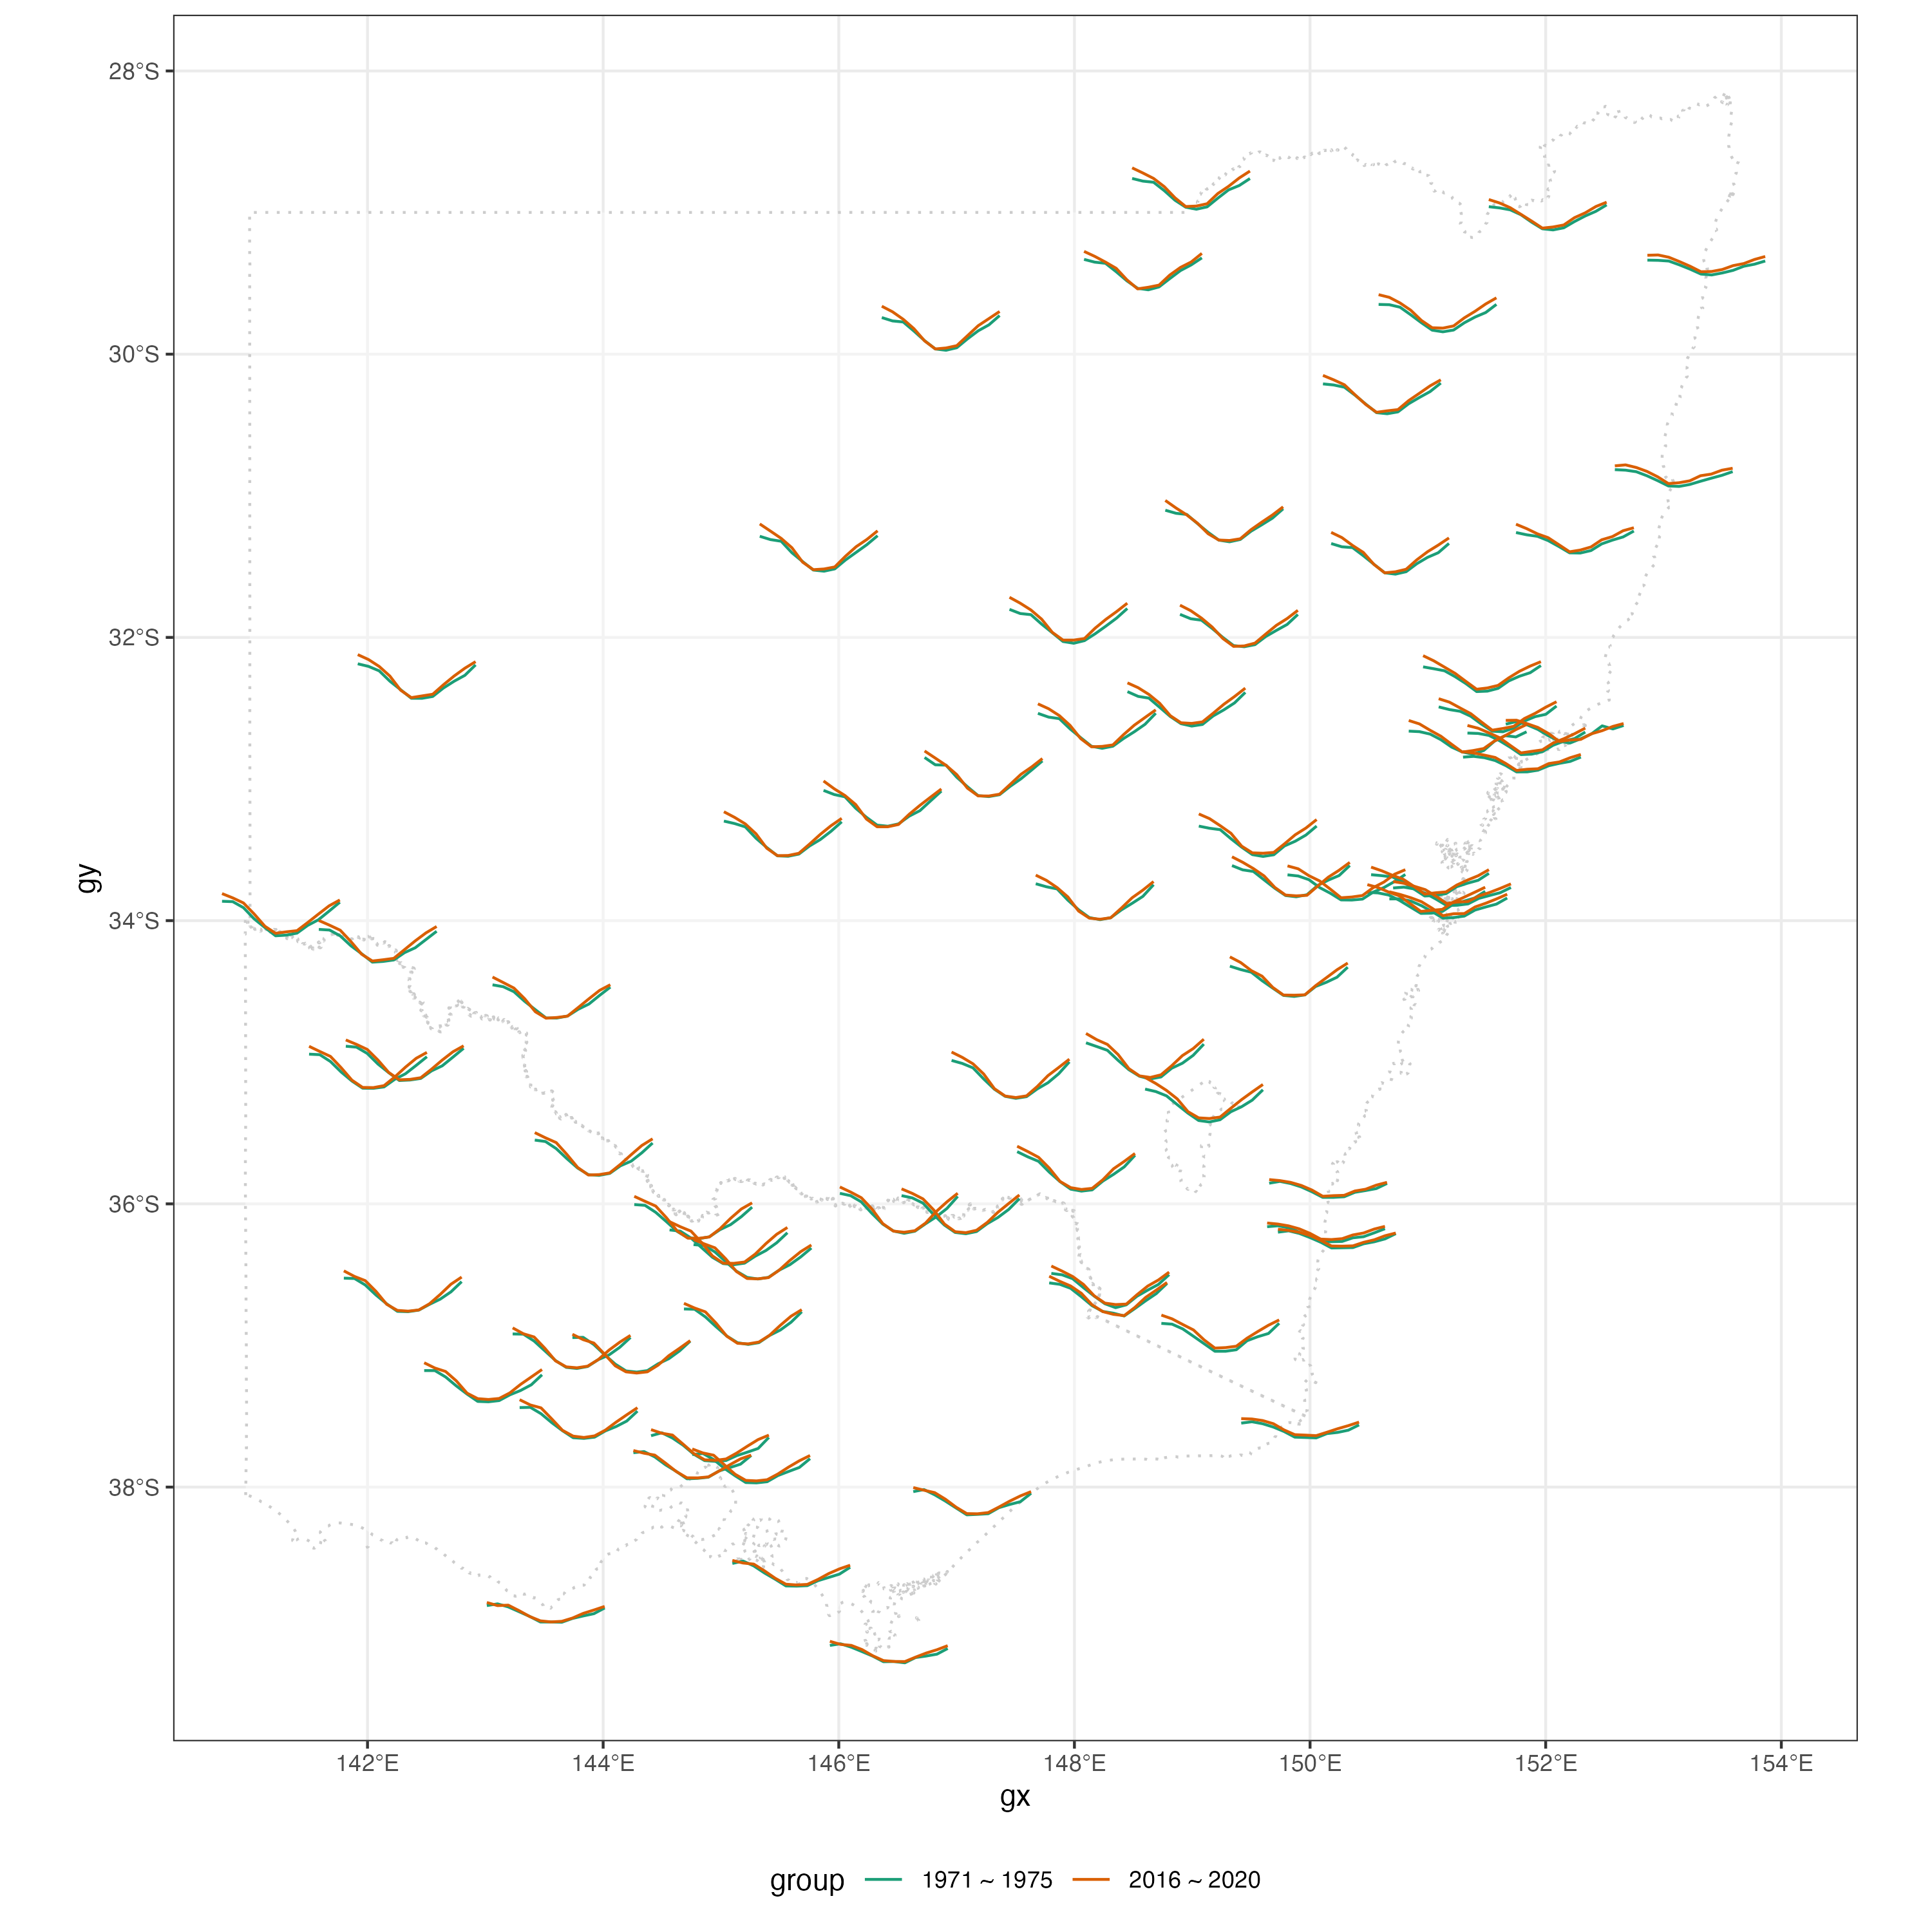
\includegraphics[width=1\linewidth,height=0.7\textheight]{figures/basic-manip} 

}

\caption[A glyph map of the mean maximum temperature by month for Victoria and New South Wales weather stations in Australia]{A glyph map of the mean maximum temperature by month for Victoria and New South Wales weather stations in Australia. On the top left corner is an insetted plot of station Cobar, which is highlighted in the black box.}\label{fig:basic-manip}
\end{figure}
\end{CodeChunk}

\hypertarget{australia-precipitation-pattern-in-2020}{%
\subsection{Australia precipitation pattern in
2020}\label{australia-precipitation-pattern-in-2020}}

In the previous example, there has already been some overlapping of the
glyphs for a few stations near (151E, 34S) and (152E, 33S) and this will
be a problem when mapping more stations in the national level.
Aggregation can be helpful to group series into clusters before
visualising the cluster with glyph map.

This example shows how to organise data at both level with
\code{switch_key()}. The dataset used is
\code{weatherdata::climate_full}, which records daily precipitation and
maximum/ minimum temperature for
\code{r nrow(weatherdata::climate_full)} stations in Australia from 2016
to 2020. A simple kmean algorithm based on the distance matrix is used
here to create 20 clusters. This creates \code{station_nested} as a
station level nested cubble with a cluster column indicating the group
each station belongs to. More complex algorithms can be used for other
problem, as long as there is a mapping from each station to a cluster.

\begin{CodeChunk}
\begin{CodeInput}
R> station_nested <- weatherdata::climate_full %>% 
+   mutate(cluster = ...)
\end{CodeInput}
\end{CodeChunk}

To create a group level cubble, use \code{switch_key()} with the new key
variable, \code{cluster}:

\begin{CodeChunk}
\begin{CodeInput}
R> cluster_nested <- station_nested %>% switch_key(cluster) 
\end{CodeInput}
\end{CodeChunk}

With the group level cubble, \code{get_centroid()} is useful to compute
the centroid of each cluster, which will be used as the major axis for
the glyph map later:

\begin{CodeChunk}
\begin{CodeInput}
R> cluster_nested <- cluster_nested %>% get_centroid()
\end{CodeInput}
\end{CodeChunk}

Long form cubble at both levels can be access through stretching the
nested form and operations applicable to long form cubble are still
available. With access to both station and cluster level cubbles,
various plots can be made to understand the cluster. Figure
\ref{fig:basic-agg} shows two example plots that can be made with this
data: subplot A makes a glyph map with cluster level cubble and subplot
B inspects the station membership of each cluster using the nested
station level cubble.

\begin{CodeChunk}
\begin{figure}

{\centering 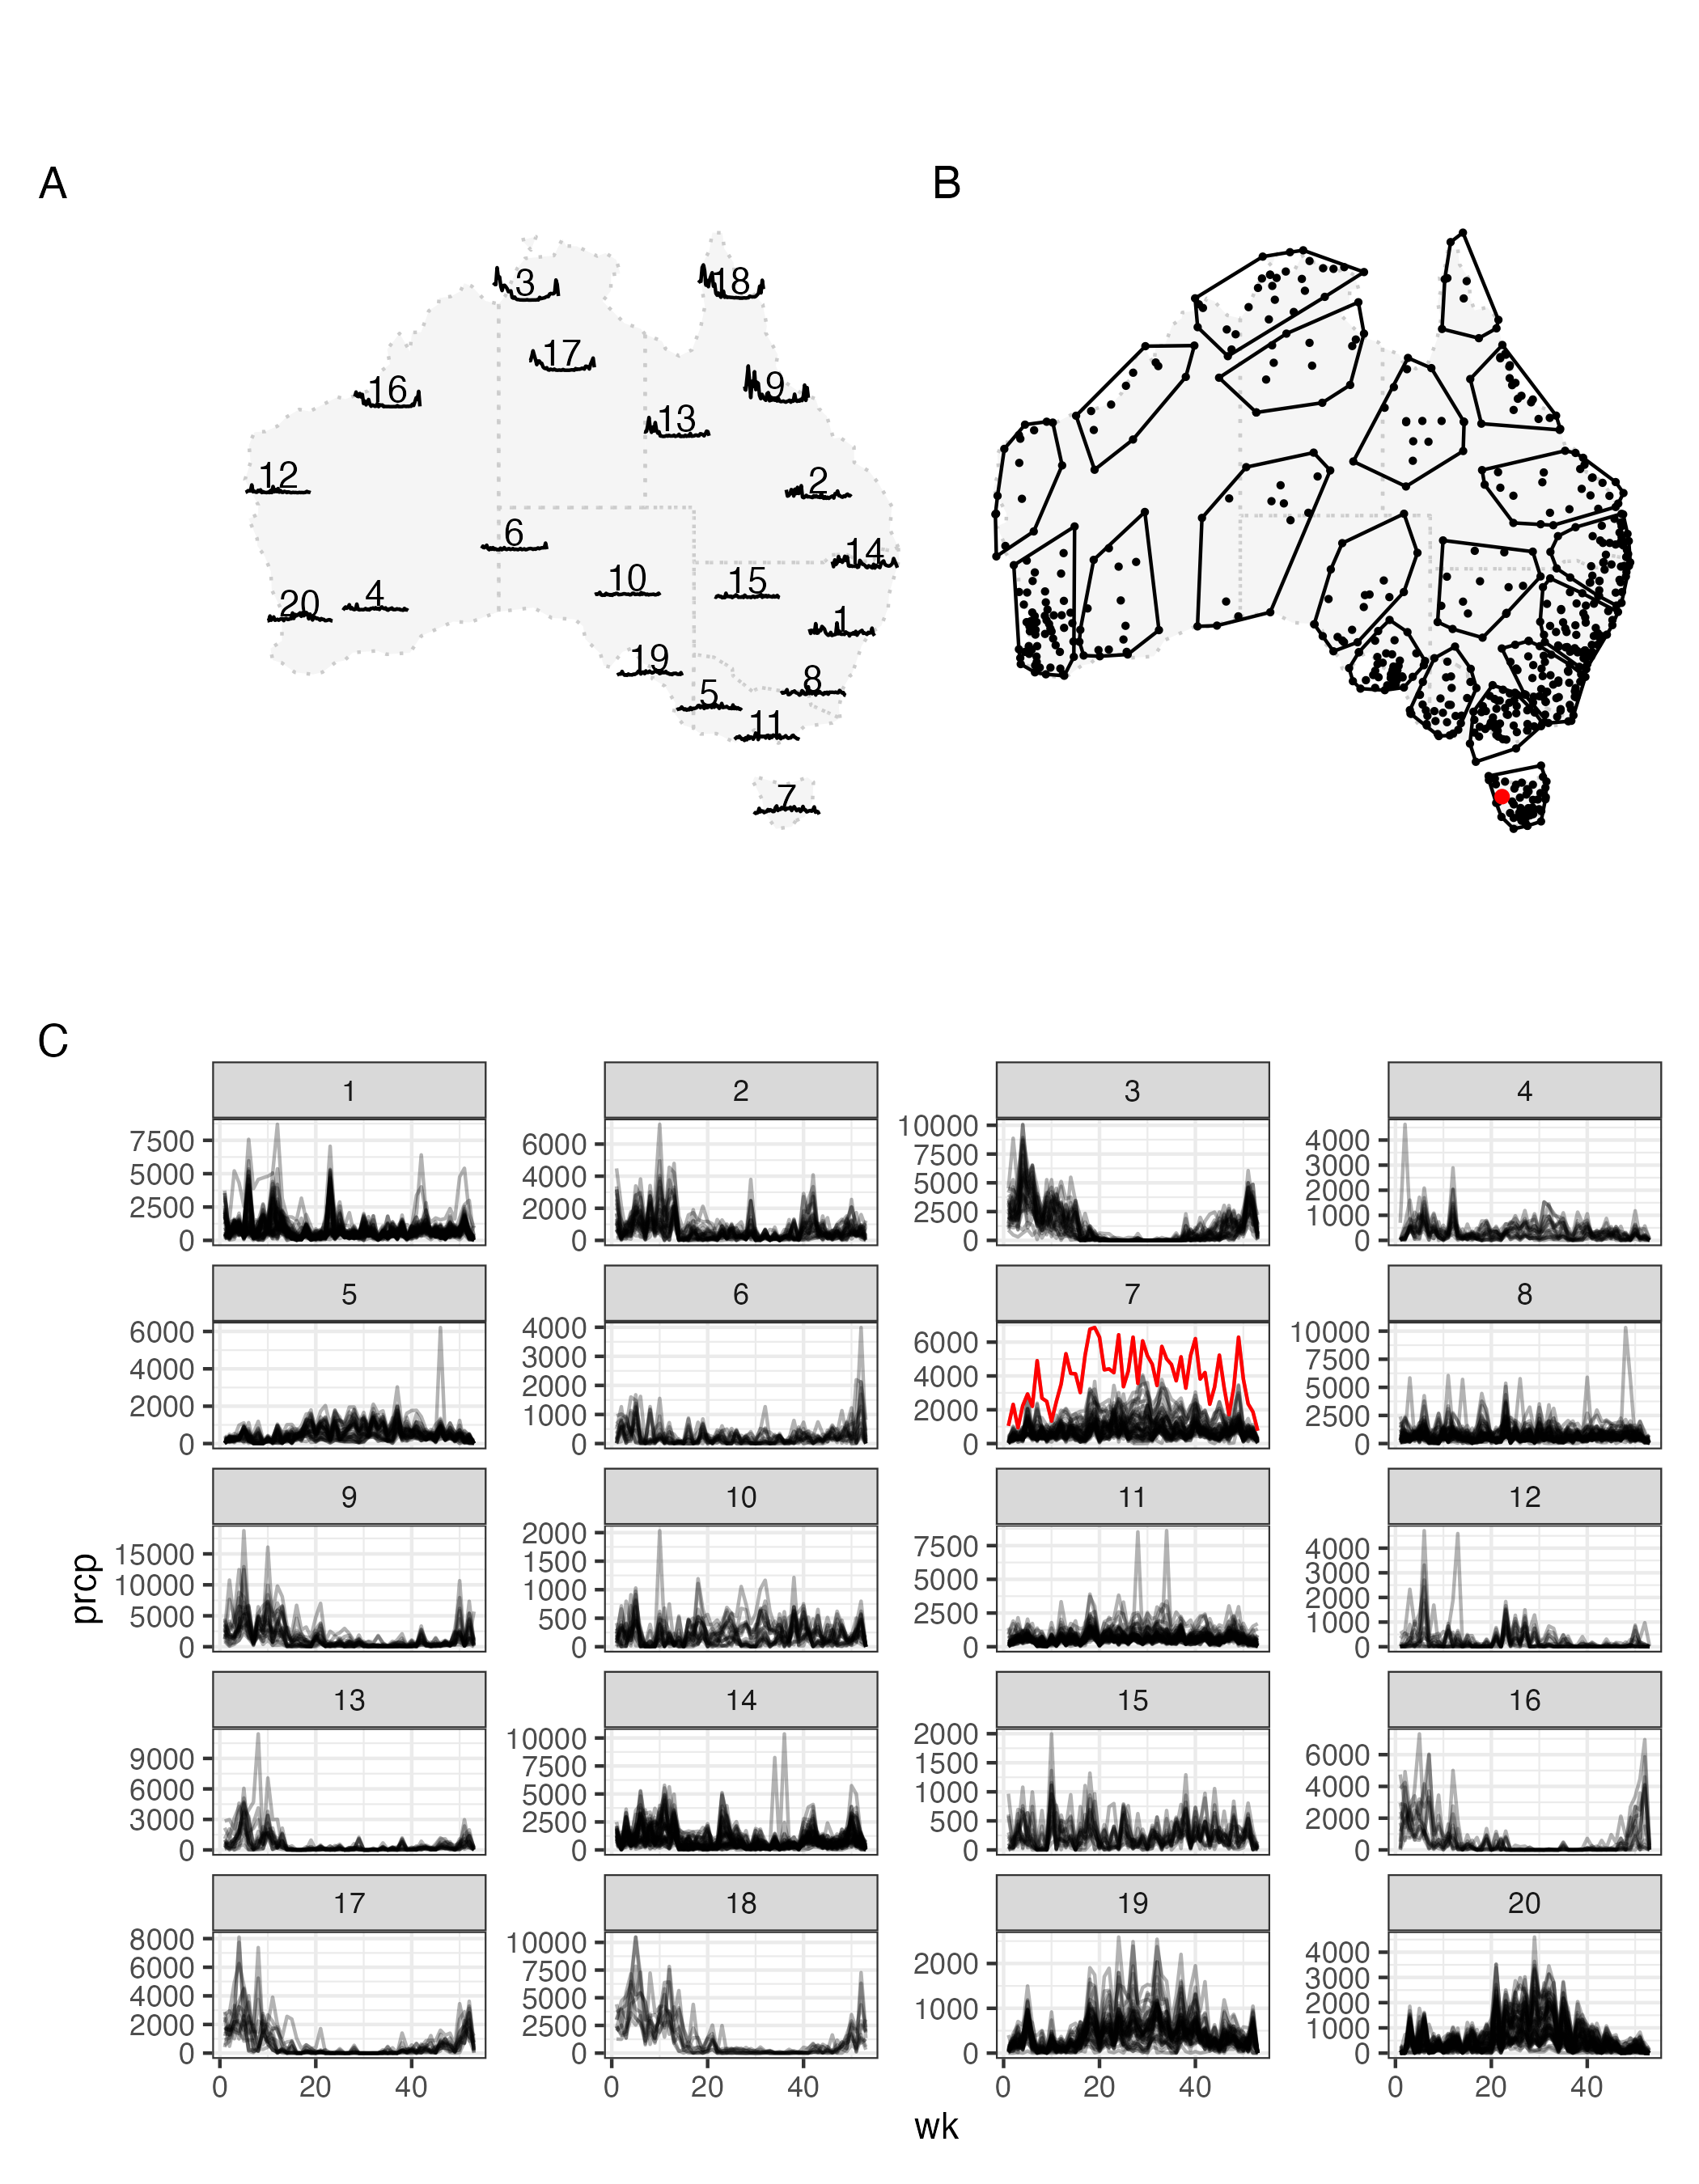
\includegraphics[width=1\linewidth]{figures/basic-agg} 

}

\caption[Profile of aggregated precipitation from 639 weather stations in Australia]{Profile of aggregated precipitation from 639 weather stations in Australia. Subplot A shows the glyph map of the weekly averaged precipitation of each cluster. The group number of printed in the middle of y minor axis and can be used as a reference line to read the magnitude of precipitation. Subplot B shows the station membership of each cluster}\label{fig:basic-agg}
\end{figure}
\end{CodeChunk}

\hypertarget{river-level-data-in-victria-water-gauges}{%
\subsection{River level data in Victria water
gauges}\label{river-level-data-in-victria-water-gauges}}

Bureau of Meteorology also collects
\href{http://www.bom.gov.au/metadata/catalogue/19115/ANZCW0503900528?template=full}{water
data} from river gauges, which includes electrical conductivity,
turbidity, water course discharge, water course level, and water
temperature. In particular, water level will interactive with
precipitation from the climate data since rainfall will raise the water
level in the river. Figure \ref{fig:matching-map} gives the location of
available weather station and water gauges in Victoria.

\begin{CodeChunk}
\begin{figure}

{\centering 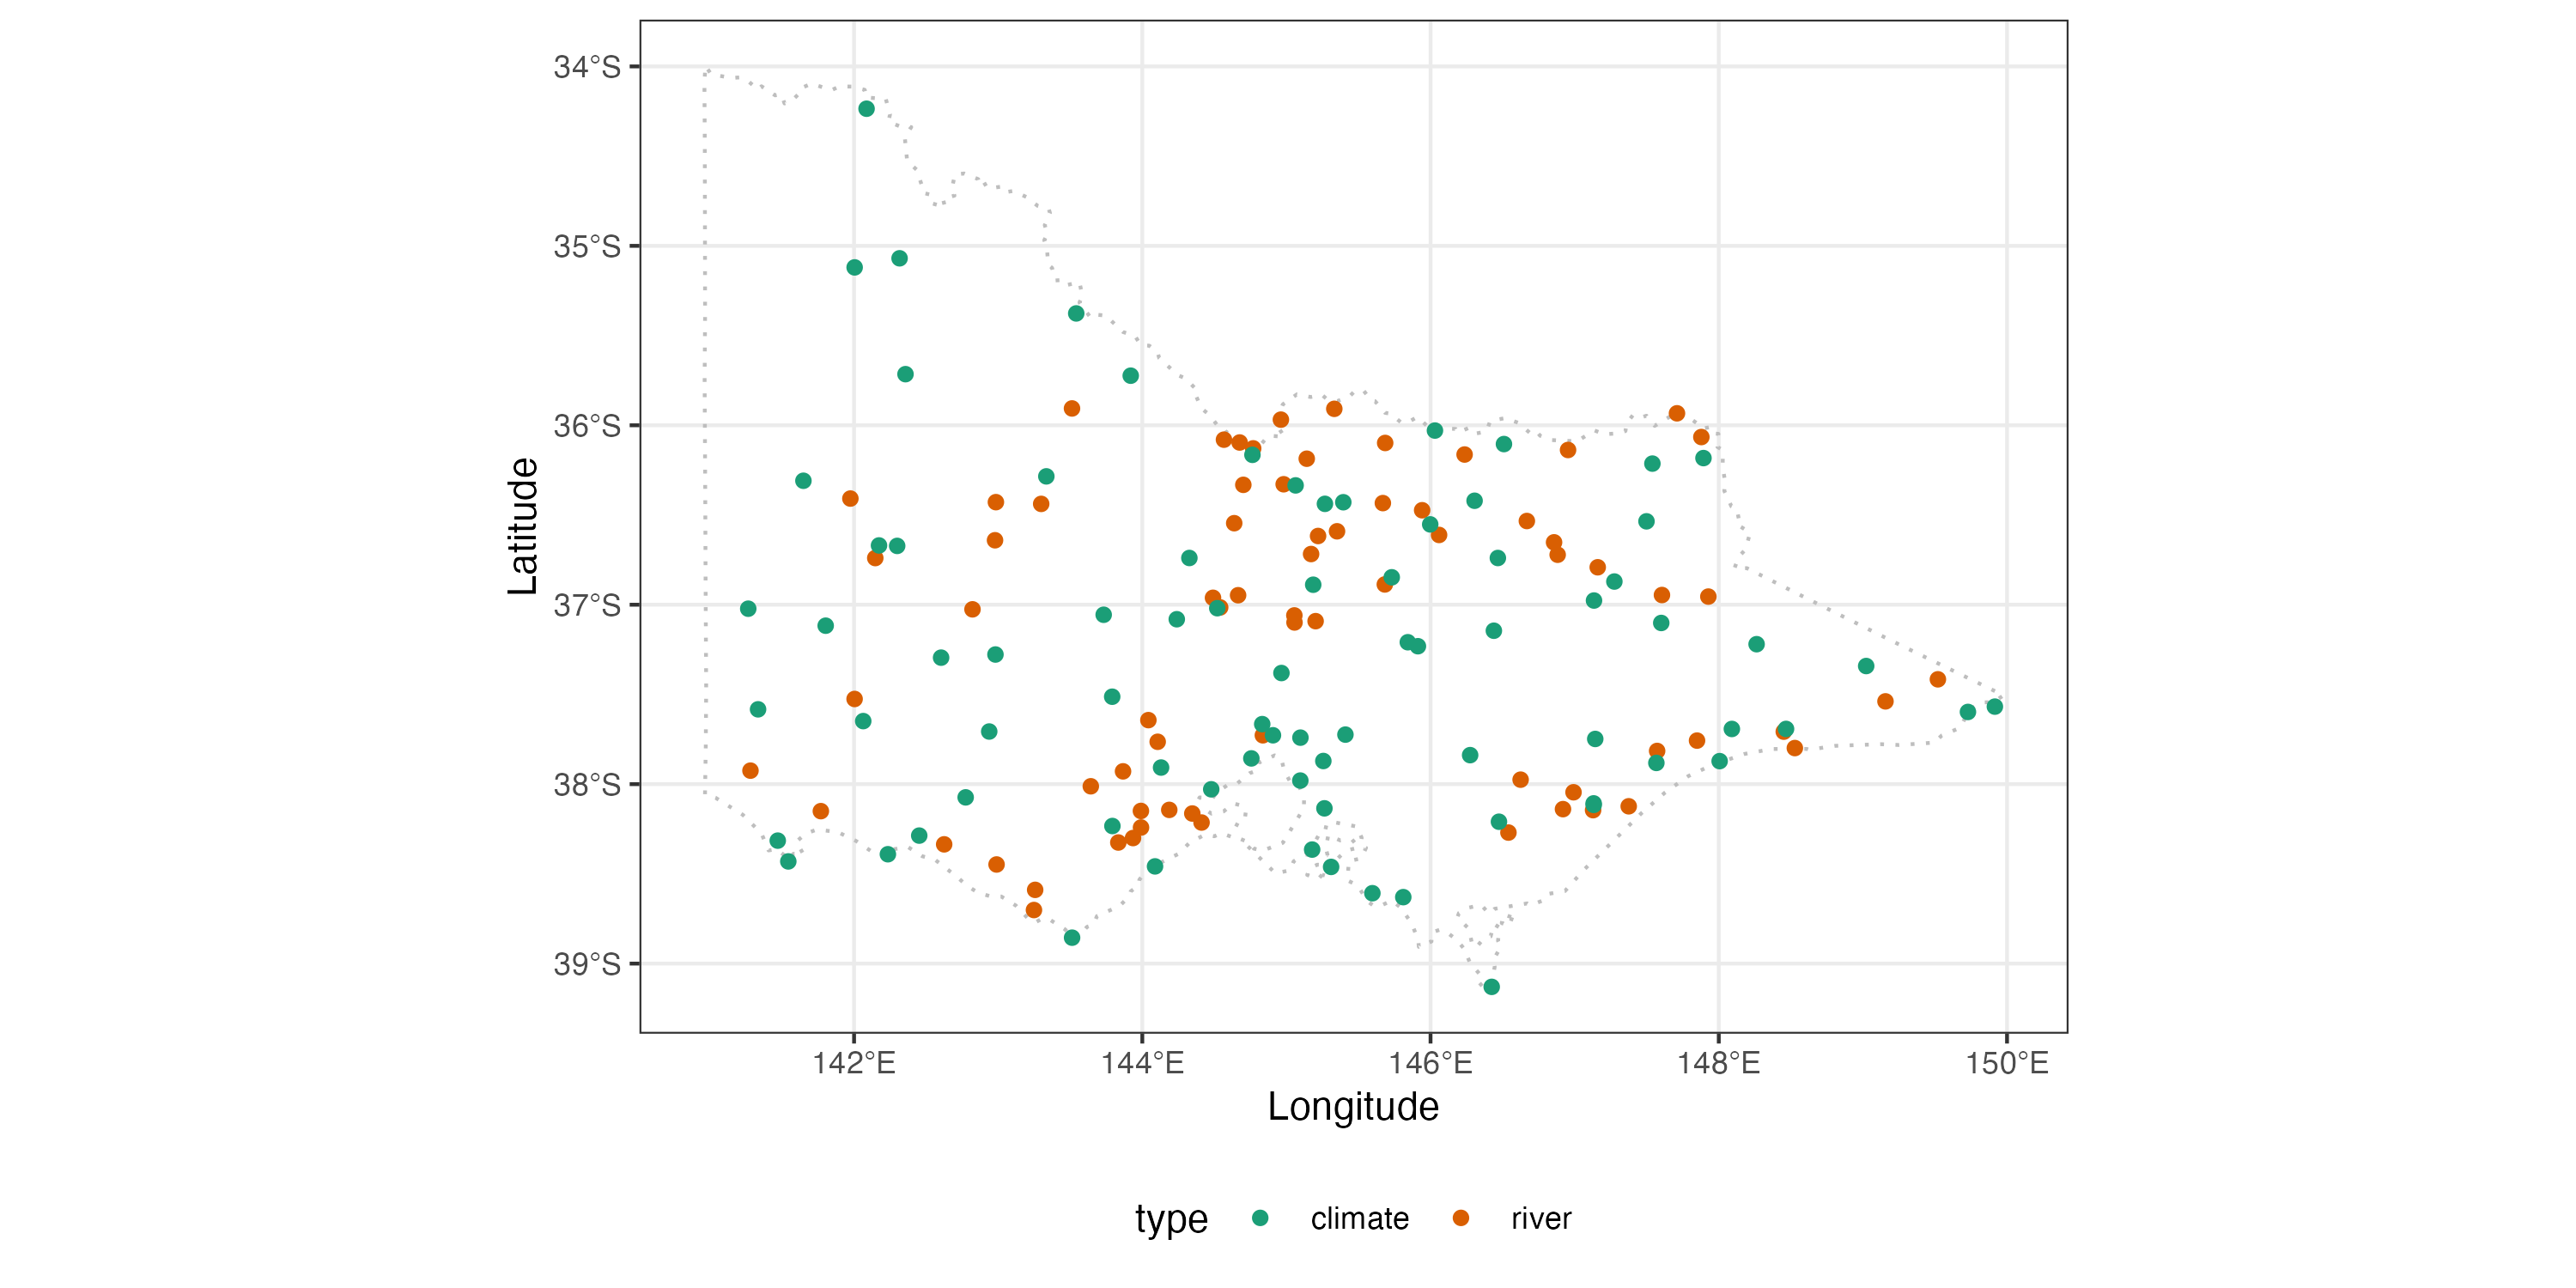
\includegraphics[width=1\linewidth]{figures/matching-map} 

}

\caption[Location of climate station and river gauges in Victoria, Australia]{Location of climate station and river gauges in Victoria, Australia.}\label{fig:matching-map}
\end{figure}
\end{CodeChunk}

From the map, a few water gauges and weather stations are close to each
other and there is the potential that fluctuation of the water level can
reflect the precipitation measured by the climate station. As introduced
in Section 3.2, \code{match_sites()} can be used to match one source of
data with another source in a cubble. Here \code{prcp} in \code{climate}
will be matched to \code{Water_course_level} in \code{river}, which is
specified in the argument \code{temporal_var_to_match}.
\code{temporal_independent} controls the dataset that will be used to
construct the interval (see the illustration in section 3.2 for details
on this). Here the goal is to see if precipitation will be reflected by
the water level in the river and hence a lagged effect of water level on
precipitation. This will put precipitation data, \code{climate}, as the
independent. Given there is one year worth of data, the number of peak
(\code{temporal_n_highest}) to consider is slightly raised from a
default 20 to 30. \code{temporal_min_match} filters out pairs don't have
enough match and to return all the pairs, set \code{temporal_min_match}
to 0.

\begin{CodeChunk}
\begin{CodeInput}
R> res <- match_sites(
+   river, climate,
+   temporal_var_to_match = c("Water_course_level" = "prcp"),
+   temporal_independent = "prcp",  
+   temporal_n_highest = 30,
+   temporal_min_match = 15
+ )
\end{CodeInput}
\end{CodeChunk}

The output from matching is also a cubble, with additional column
\code{dist} and \code{group} produced from spatial matching and
\code{n_match} from the temporal matching.

\begin{CodeChunk}
\begin{CodeOutput}
# cubble:   id [8]: nested form
# bbox:     [144.52, -37.73, 146.06, -36.55]
# temporal: date [date], matched_var [dbl]
  id          name                lat  long type    dist group ts        n_match
  <chr>       <chr>             <dbl> <dbl> <chr>  <dbl> <int> <list>      <int>
1 405234      SEVEN CREEKS @ D~ -36.9  146. river   6.15     5 <tibble ~      21
2 404207      HOLLAND CREEK @ ~ -36.6  146. river   8.54    10 <tibble ~      21
3 ASN00082042 strathbogie       -36.8  146. clima~  6.15     5 <tibble ~      21
4 ASN00082170 benalla airport   -36.6  146. clima~  8.54    10 <tibble ~      21
5 230200      MARIBYRNONG RIVE~ -37.7  145. river   6.17     6 <tibble ~      19
6 ASN00086038 essendon airport  -37.7  145. clima~  6.17     6 <tibble ~      19
7 406213      CAMPASPE RIVER @~ -37.0  145. river   1.84     1 <tibble ~      18
8 ASN00088051 redesdale         -37.0  145. clima~  1.84     1 <tibble ~      18
\end{CodeOutput}
\end{CodeChunk}

Figure \ref{fig:matching} plots the matched pairs on the map or to view
the matched series and with the chosen parameter, there are four pairs
of matches, which all locates in the middle Victoria and the concurrent
increase of precipitation and water level can be observed.

\begin{CodeChunk}
\begin{figure}

{\centering 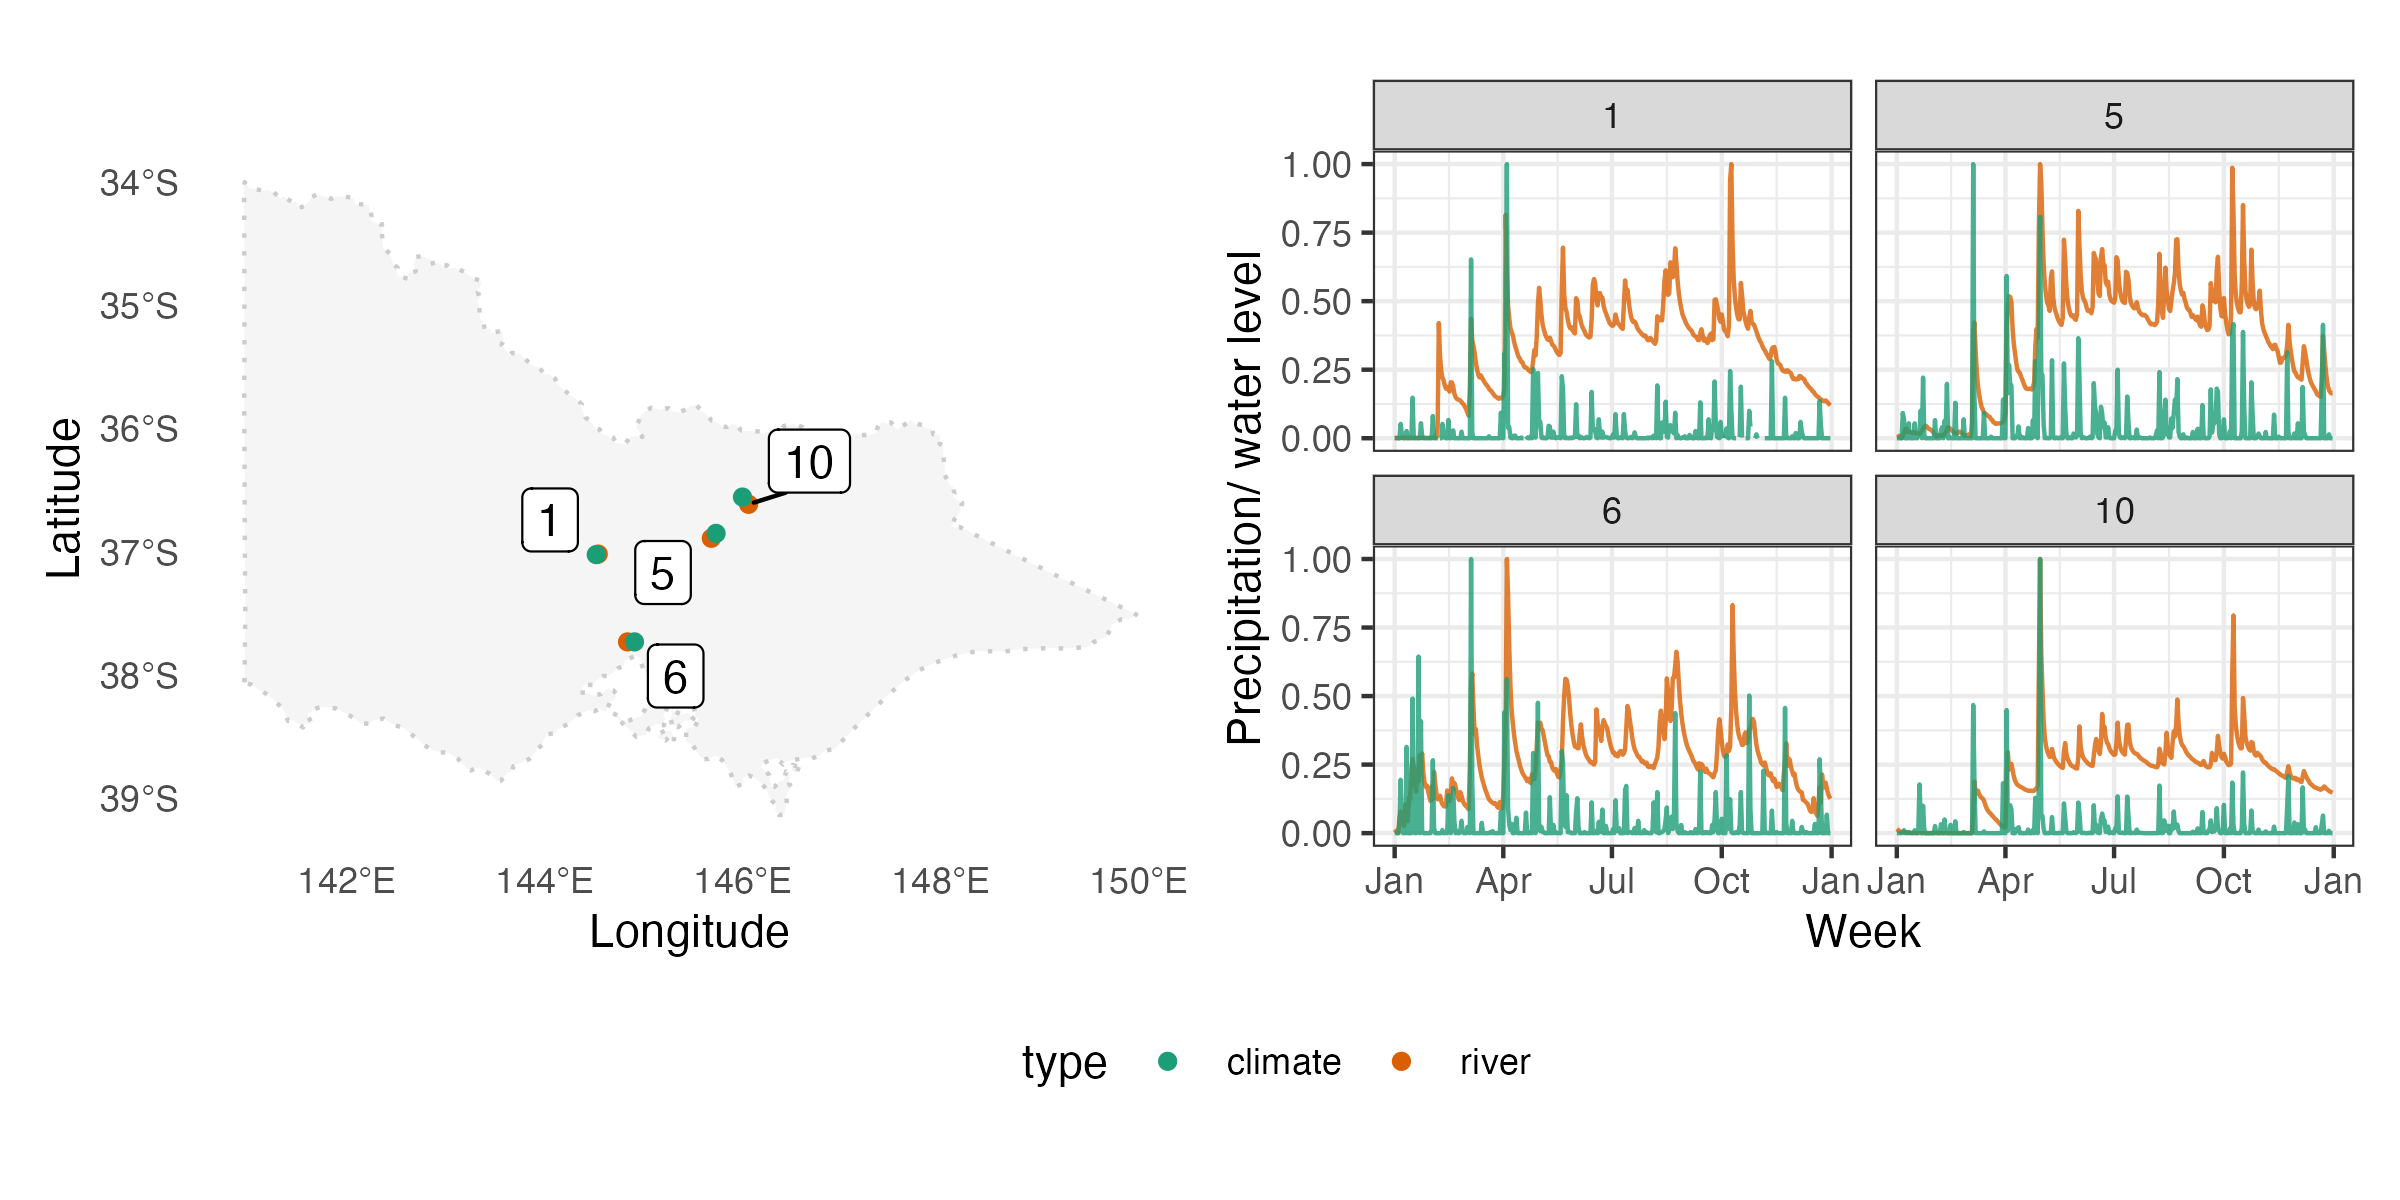
\includegraphics[width=1\linewidth]{figures/matching} 

}

\caption[Matched weather stations and river gauges on the map (A) and across time (B)]{Matched weather stations and river gauges on the map (A) and across time (B). Precipitation and water level have been standardised between 0 and 1 to be displayed on the same scale. The increases in the precipitation is reflected well by the water level.}\label{fig:matching}
\end{figure}
\end{CodeChunk}

\hypertarget{era5-climate-reanalysis-data}{%
\subsection{ERA5: climate reanalysis
data}\label{era5-climate-reanalysis-data}}

NetCDF (Network Common Data Form) is a data format commonly used in
climatology community to deliver global mapping of atmosphere, ocean,
and land. It has two major components: dimension to define the
spatiotemporal grid (longitude, latitude, and time) and variable which
populates the defined grid. Attributes are usually associated with
dimension and variable in the NetCDF format data and a
\href{http://cfconventions.org/}{metadata convention for climate and
forecast} has been designed to standardise this data format. Current
packages on manipulating NetCDF data in R include a high-level R
interface: \pkg{ncdf4} \citep{ncdf4}, a low-level interface that calls
C-interface: \pkg{RNetCDF} \citep{rnetcdf, michna2013rnetcdf}, and a
tidyverse implementation: \pkg{tidync} \citep{tidync}.

Cubble provides an \code{as_cubble()} method to coerce the \code{ncdf4}
class from the \pkg{ncdf4} package into a \code{cubble}. It maps each
combination of longitude and latitude into an \code{id} (the \code{key})
and nests time and variables in the nested form:

\begin{CodeChunk}
\begin{CodeInput}
R> # read in the .nc file as a ncdf4 class
R> raw <- ncdf4::nc_open(here::here("data/era5-pressure.nc"))
R> 
R> # convert the variable q and z in the ncdf4 into a cubble
R> dt <- as_cubble(raw, vars = c("q", "z"))
\end{CodeInput}
\end{CodeChunk}

Memory limit with Netcdf data in cubble depends on longitude grid point
x latitude grid point x time grid point x number of variable. Cubble can
handle slightly more than 300 x 300 (longitude x longitude) grid points
for 3 variables in one year and spatial grid can be reduced to trade for
longer time period and more variables. A 300 by 300 spatial grid can be
a bounding box of {[}100, -80, 180, 0{]} at 0.25 degree resolution or
global bounding box {[}-180, -90, 180, -90{]} at 1 degree resolution.
Subsetting longitude and latitude grid is available through
\code{long_range} and \code{lat_range} if the Netcdf file has finer
resolution than needed.

\begin{CodeChunk}
\begin{CodeInput}
R> # Assume \code{my_ncdf} has bounding box of [-180, -90, 180, -90] 
R> # at 0.25 degree resolution and subset it to have 
R> # 1 degree resolution:
R> dt <- as_cubble(my_ncdf, vars = c("q", "z"), 
+                 long_range = seq(-180, 180, 1), 
+                 lat_range = seq(-90, 90, 1))
\end{CodeInput}
\end{CodeChunk}

Figure \ref{fig:netcdf} gives an example of reproducing Figure 19 in
\citet{hersbach2020era5} using ERA5 data. ERA5 data
\citep{hersbach2020era5} is the latest reanalysis of global atmosphere,
land surface, and ocean waves from 1950 onwards and is available in the
NetCDF format. It can be directly downloaded from the
\href{https://cds.climate.copernicus.eu/cdsapp\#!/dataset/reanalysis-era5-pressure-levels?tab=overview}{Copernicus
Climate Data Store (CDS)} website or programmatically via R package
\pkg{ecmwfr} \citep{ecwmfr}. Variable Specific humidity and geopotential
are queried on the 10 hPa pressure level for four dates: 2002-09-22,
2002-09-26, 2002-09-30, and 2002-10-04 and once downloaded, the data can
be read into a cubble using the code above. Readers who are interested
in the details of can refer to \citet{simmons2020global} and
\citet{simmons2005ecmwf}.

\begin{CodeChunk}
\begin{figure}

{\centering 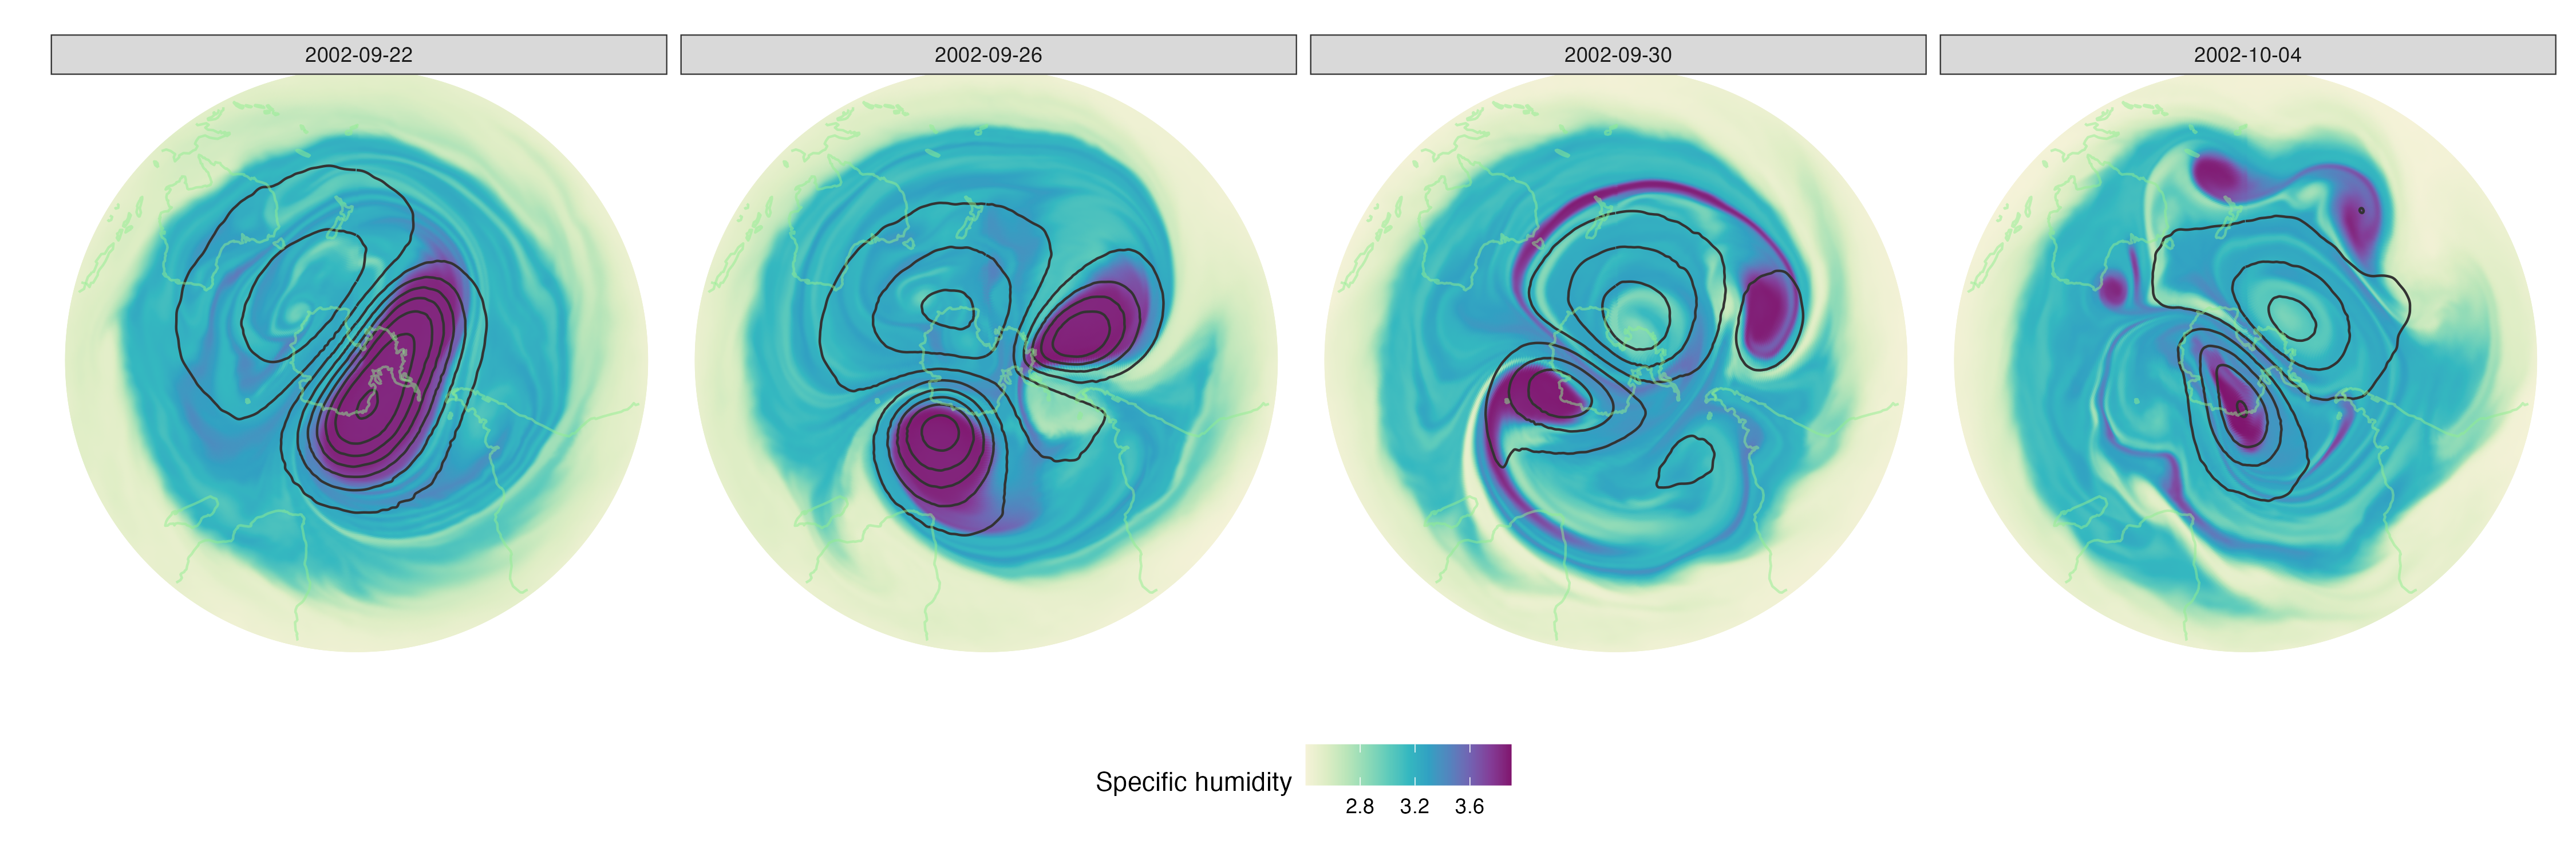
\includegraphics[width=1\linewidth]{/Users/sherryzhang/Documents/research/paper-cubble/figures/netcdf} 

}

\caption[A reproduction of the second row of Figure 19 in  Hersbach (2020)]{A reproduction of the second row of Figure 19 in  Hersbach (2020).}\label{fig:netcdf}
\end{figure}
\end{CodeChunk}

\hypertarget{interative-graphic-with-cubble}{%
\subsection{Interative graphic with
cubble}\label{interative-graphic-with-cubble}}

With spatio-temporal data, users may wish to make plots to learn the
spatial distribution of a variable or to find patterns such as trend or
seasonality in the time series. Combining this two types of plot with
interactivity let users to link between points on the map and their
corresponding time series and explore the spatial and temporal dimension
of the data simultaneously. Below is an example that describes the
process of building an interactive graphic with \pkg{cubble} and
\textbackslash pkg\{crosstalk\{.

Starting with the original data, some pre-processing may be required to
summarise the data before the visualisation. This example explores the
variation of monthly temperature range across 639 weather stations in
Australia and with \texttt{weatherdata::climate\_full}, daily
temperature range is first calculated as the difference between
\code{tmax} and \code{tmin}. The three daily variables are then averaged
into month over 2016 - 2020 in the long form. Variance of the
temperature difference is then calculated for each station in the nested
form. Then, a \code{SharedData} object is constructed for each form of
the cubble and the same \code{group} argument ensures the cross-linking
of the two forms via the common \code{id} column. The spatial map and
time series plot are then made with each \code{SharedData} objects
separately. In this example, stations on the Australia map, made from
the nested form, are coloured by the calculated variance and a ribbon
band is constructed using the long form cubble to show the maximum and
minimum temperature of each station across month. With a different
dataset, users are free to calculate any per station measure in the
nested form or to make any time-wise summary of the data in the long
form to customise the spatial or temporal view. And the cross-linking is
always safeguarded by the shared \code{id} column embedded in the cubble
structure. Below is the pseudo code that outlines the process to
construct an interactive graphic described above:

\begin{CodeChunk}
\begin{CodeInput}
R> # data pre-processing
R> clean <- weatherdata::climate_full %>% ...
R> 
R> # created SharedData instance for crosstalk
R> nested <- clean %>% SharedData$new(~id, group = "cubble")
R> long <- stretch(clean) %>% SharedData$new(~id, group = "cubble")
R> 
R> # create the spatial and temporal view each with a ShareData instance
R> p1 <- nested %>% ...
R> p2 <- long %>% ...
R> 
R> # Combine p1 and p2
R> crosstalk::bscols(plotly::ggplotly(p1), plotly::ggplotly(p2), ...)
\end{CodeInput}
\end{CodeChunk}

In Figure \ref{fig:interactive-linking}, the first row shows the initial
view of the interactive graphic. Overall, most regions in Australia have
low variance of temperature range across different months while the
north-west coastline, bottom of South Australia, and Victoria stands out
with larger monthly changes. In the second row, Mount Elizabeth is
selected on the map given its dark colour and this links to the ribbon
on the right where there is a larger temperature range is presented in
Australian winter (June to August). The third row selects the Grampian
station in Victoria and the linked ribbon shows an opposite wider range
in Australian summer period (December to February). The last row selects
point with the lowest minimum temperature in August in the ribbon plot
and surprisingly, this links to the Thredbo Airport in the Victoria and
New South Wales border, rather than somewhere in the Tasmania island!

\begin{CodeChunk}
\begin{figure}

{\centering 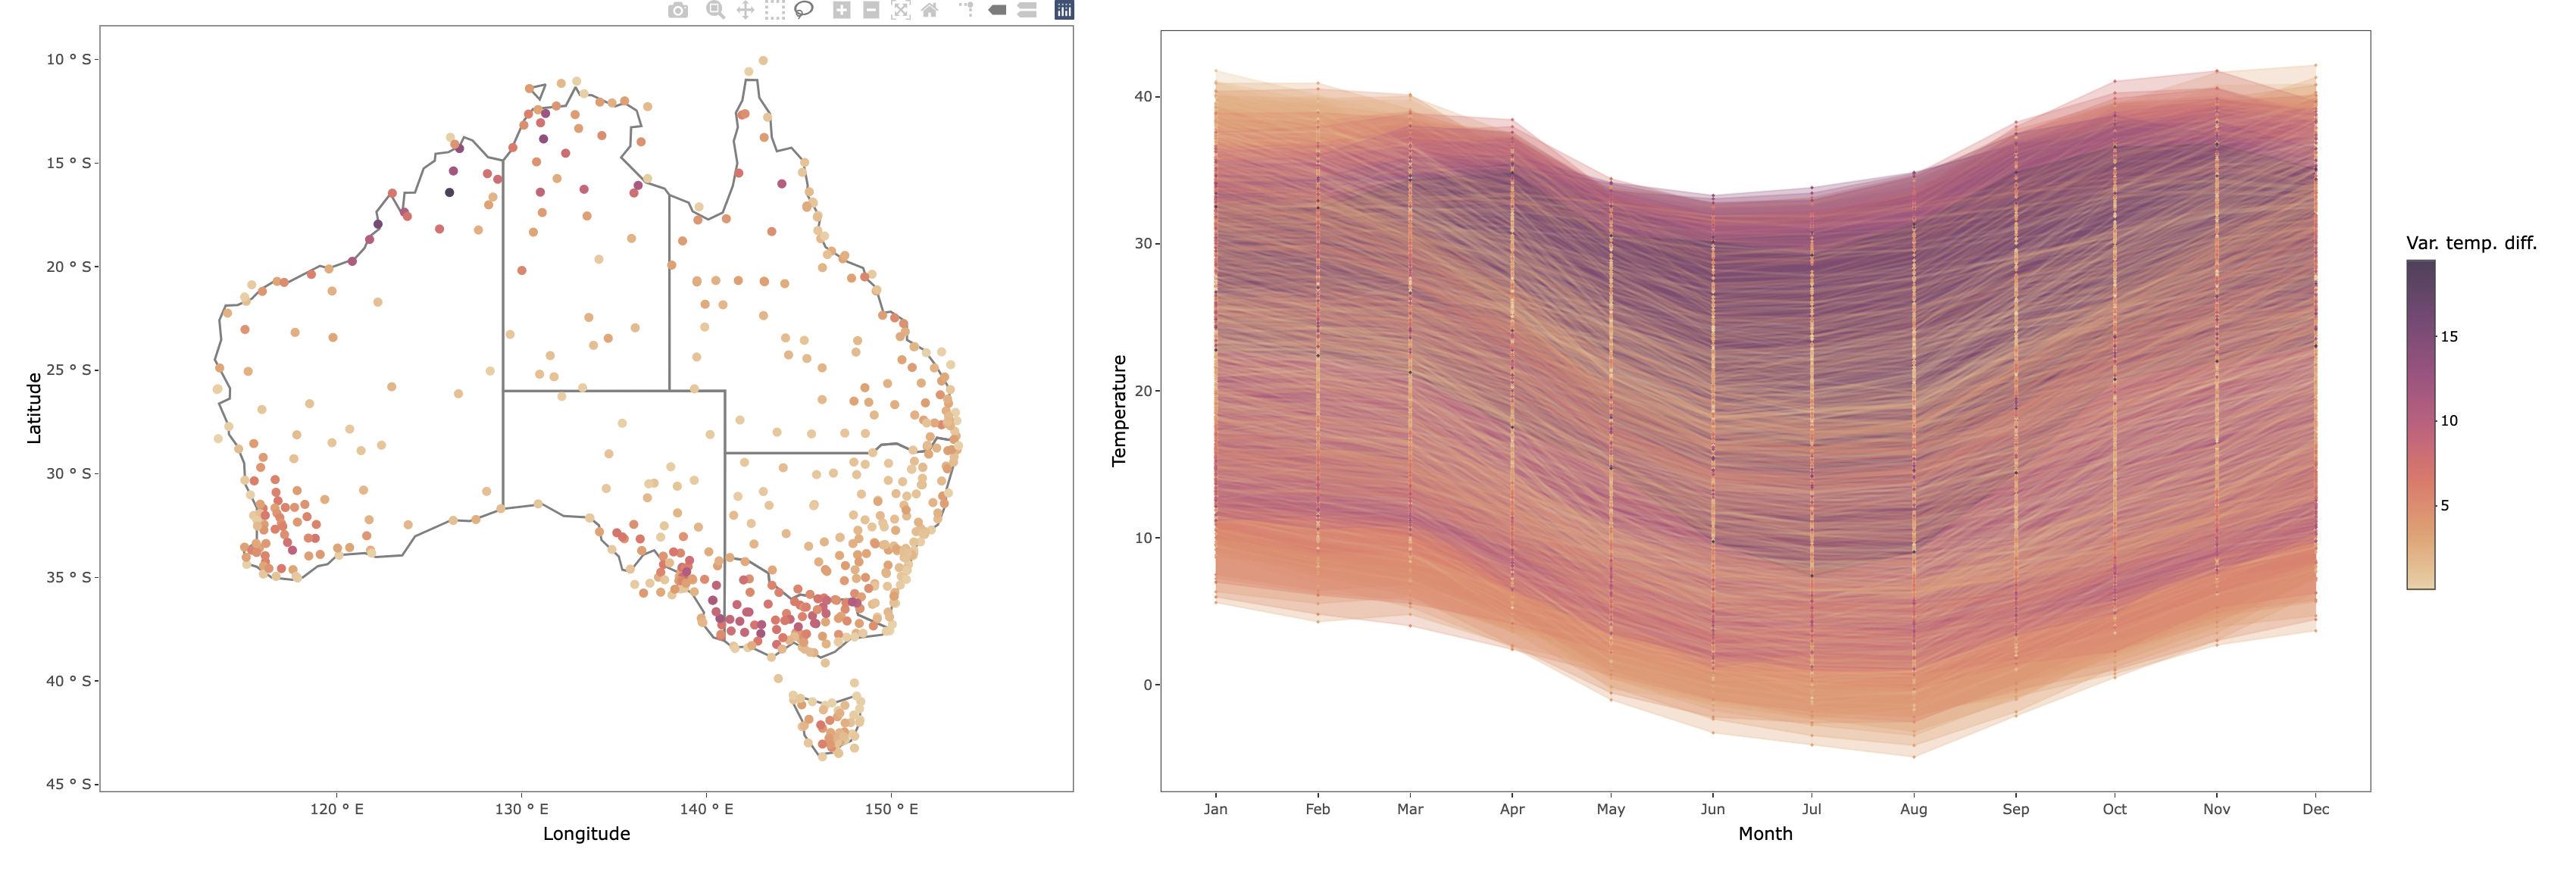
\includegraphics[width=1\linewidth,height=0.23\textheight]{/Users/sherryzhang/Documents/research/paper-cubble/figures/linking} 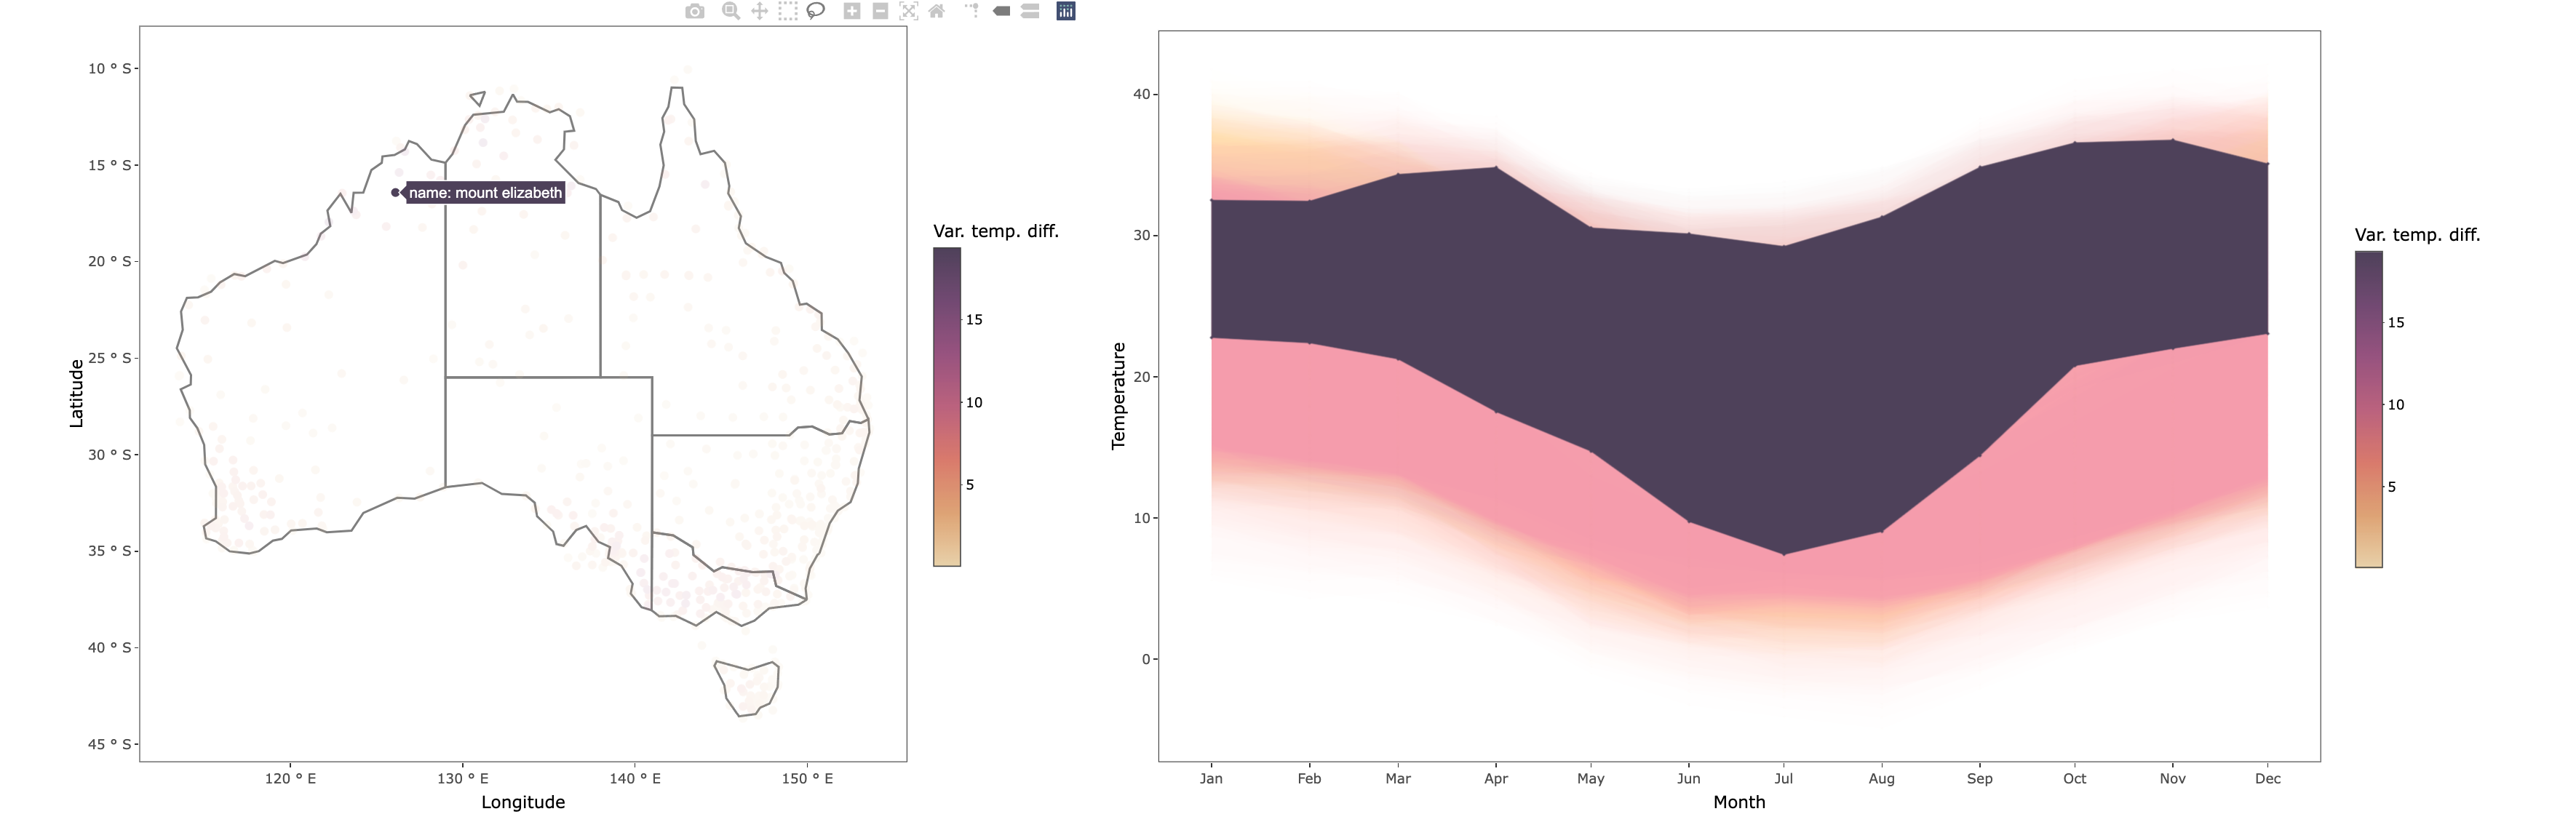
\includegraphics[width=1\linewidth,height=0.23\textheight]{/Users/sherryzhang/Documents/research/paper-cubble/figures/linking-north} 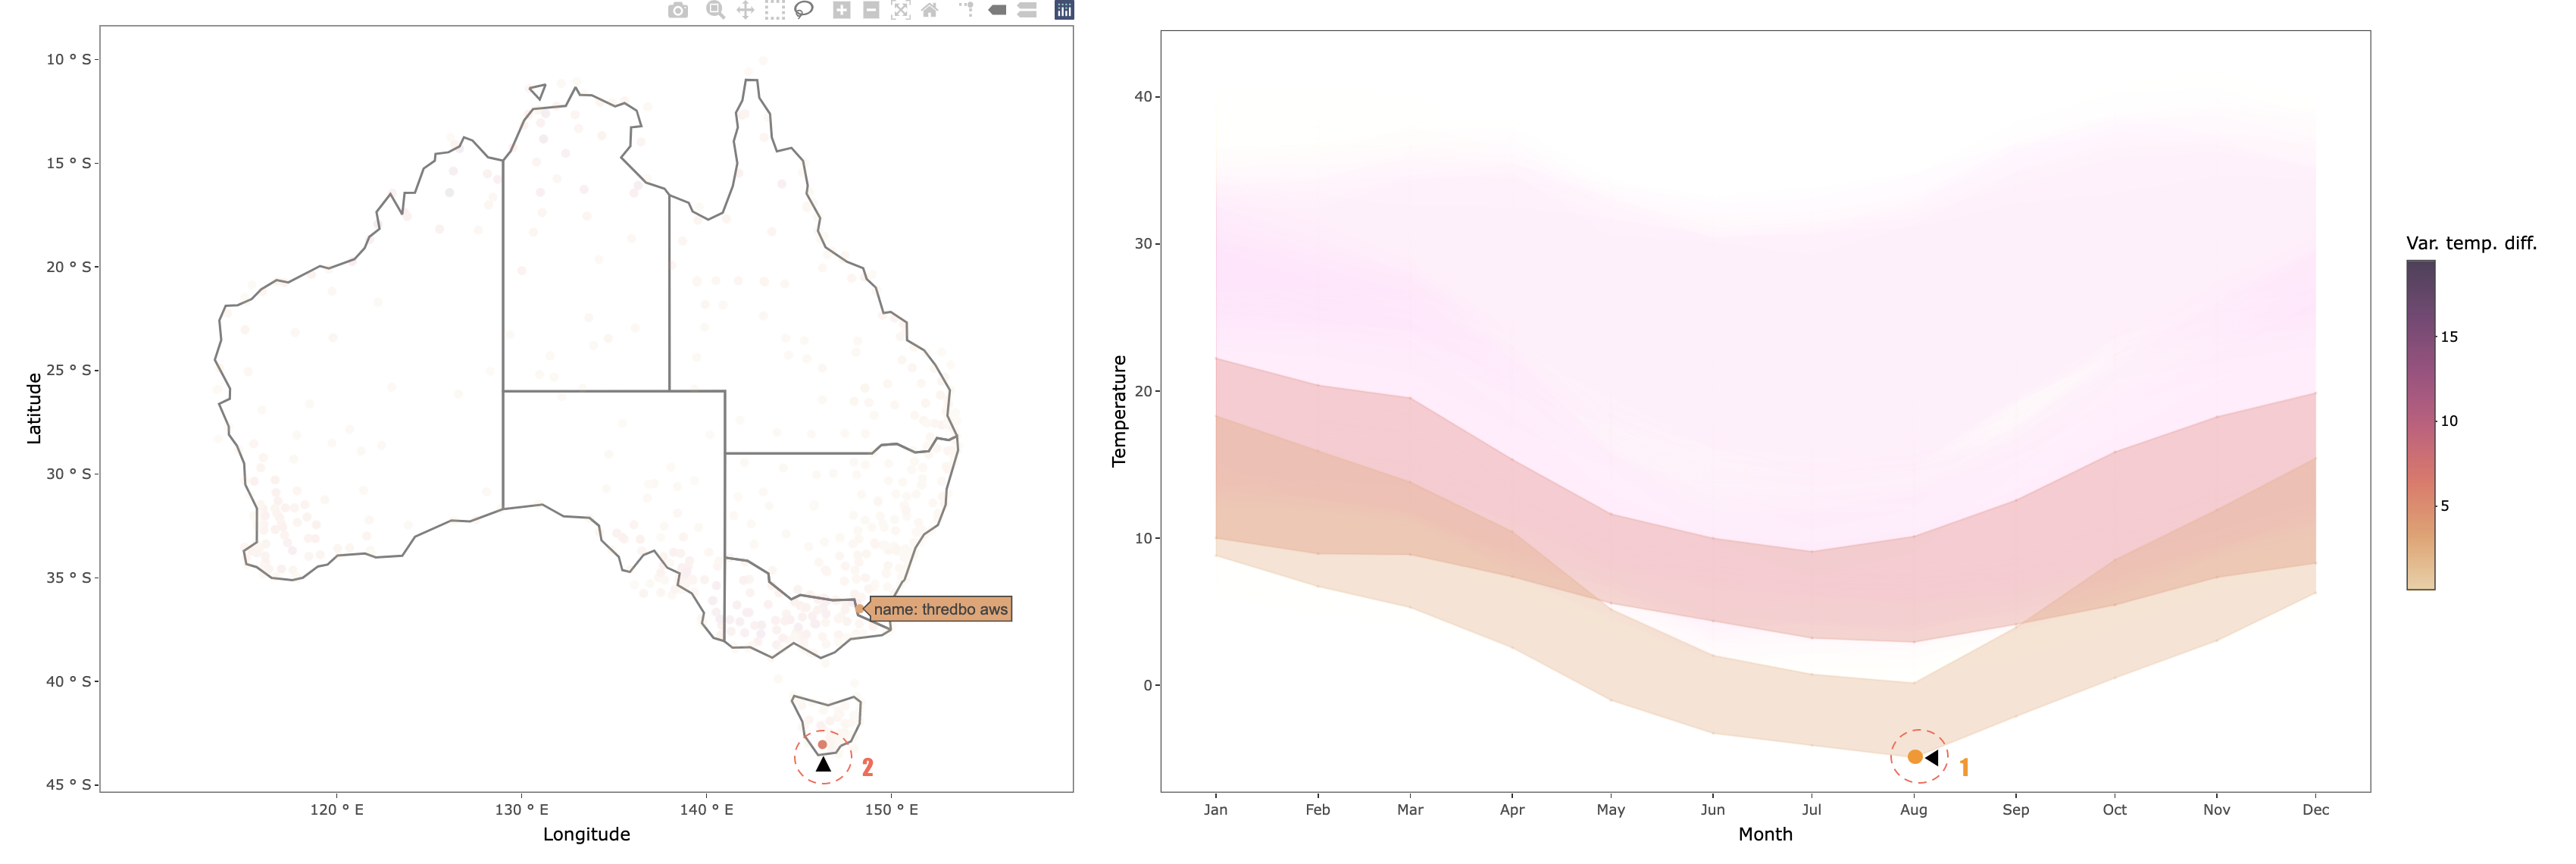
\includegraphics[width=1\linewidth,height=0.23\textheight]{/Users/sherryzhang/Documents/research/paper-cubble/figures/linking-lower} 

}

\caption[Exploring temperature variation using linking of a map and seasonal display]{Exploring temperature variation using linking of a map and seasonal display. Each row is a screen dump of the process. The top row shows all locations and all temperature profiles. Selecting a location with high variance on the map produces the plot in the second row. The maximum nad minimum temperature is shown using a ribbon. The bottom row first selects the lowest temperature in Auguest in the seasonal display. A location in the Tasmania Island is then selected and surprisingly, it is actually warmer than the Thredbo AWS.}\label{fig:interactive-linking}
\end{figure}
\end{CodeChunk}

With leaflet popup, the temperature range can be displayed as a small
subplot upon clicking on the map. This would require first creating the
popup plots from the long form cubble as a vector and then add these
plots to a leaflet map, created from the nested cubble, with
\code{leafpop::addPopupGraphs()}:

\begin{CodeChunk}
\begin{CodeInput}
R> # data pre-processing
R> clean <- weatherdata::climate_full %>% ...
R> 
R> # use the long form to create subplots for each station
R> df_id <- unique(clean$id)
R> p <- map(1:length(df_id), function(i){
+   dt <- clean %>% filter(id == df_id[i])
+   ggplot(dt) %>% ...
+ })
R> 
R> # create nested form leaflet map with temperature band as subplots 
R> nested <- tamp(clean)
R> leaflet(nested) %>% 
+   addTiles() %>% 
+   addCircleMarkers(group = "a", ...) %>% 
+   leafpop::addPopupGraphs(graph = p, ...)
\end{CodeInput}
\end{CodeChunk}

Figure \ref{fig:interactive-popup} shows the same content as Figure
\ref{fig:interactive-linking} but made with leaflet and popups.

\begin{CodeChunk}
\begin{figure}

{\centering 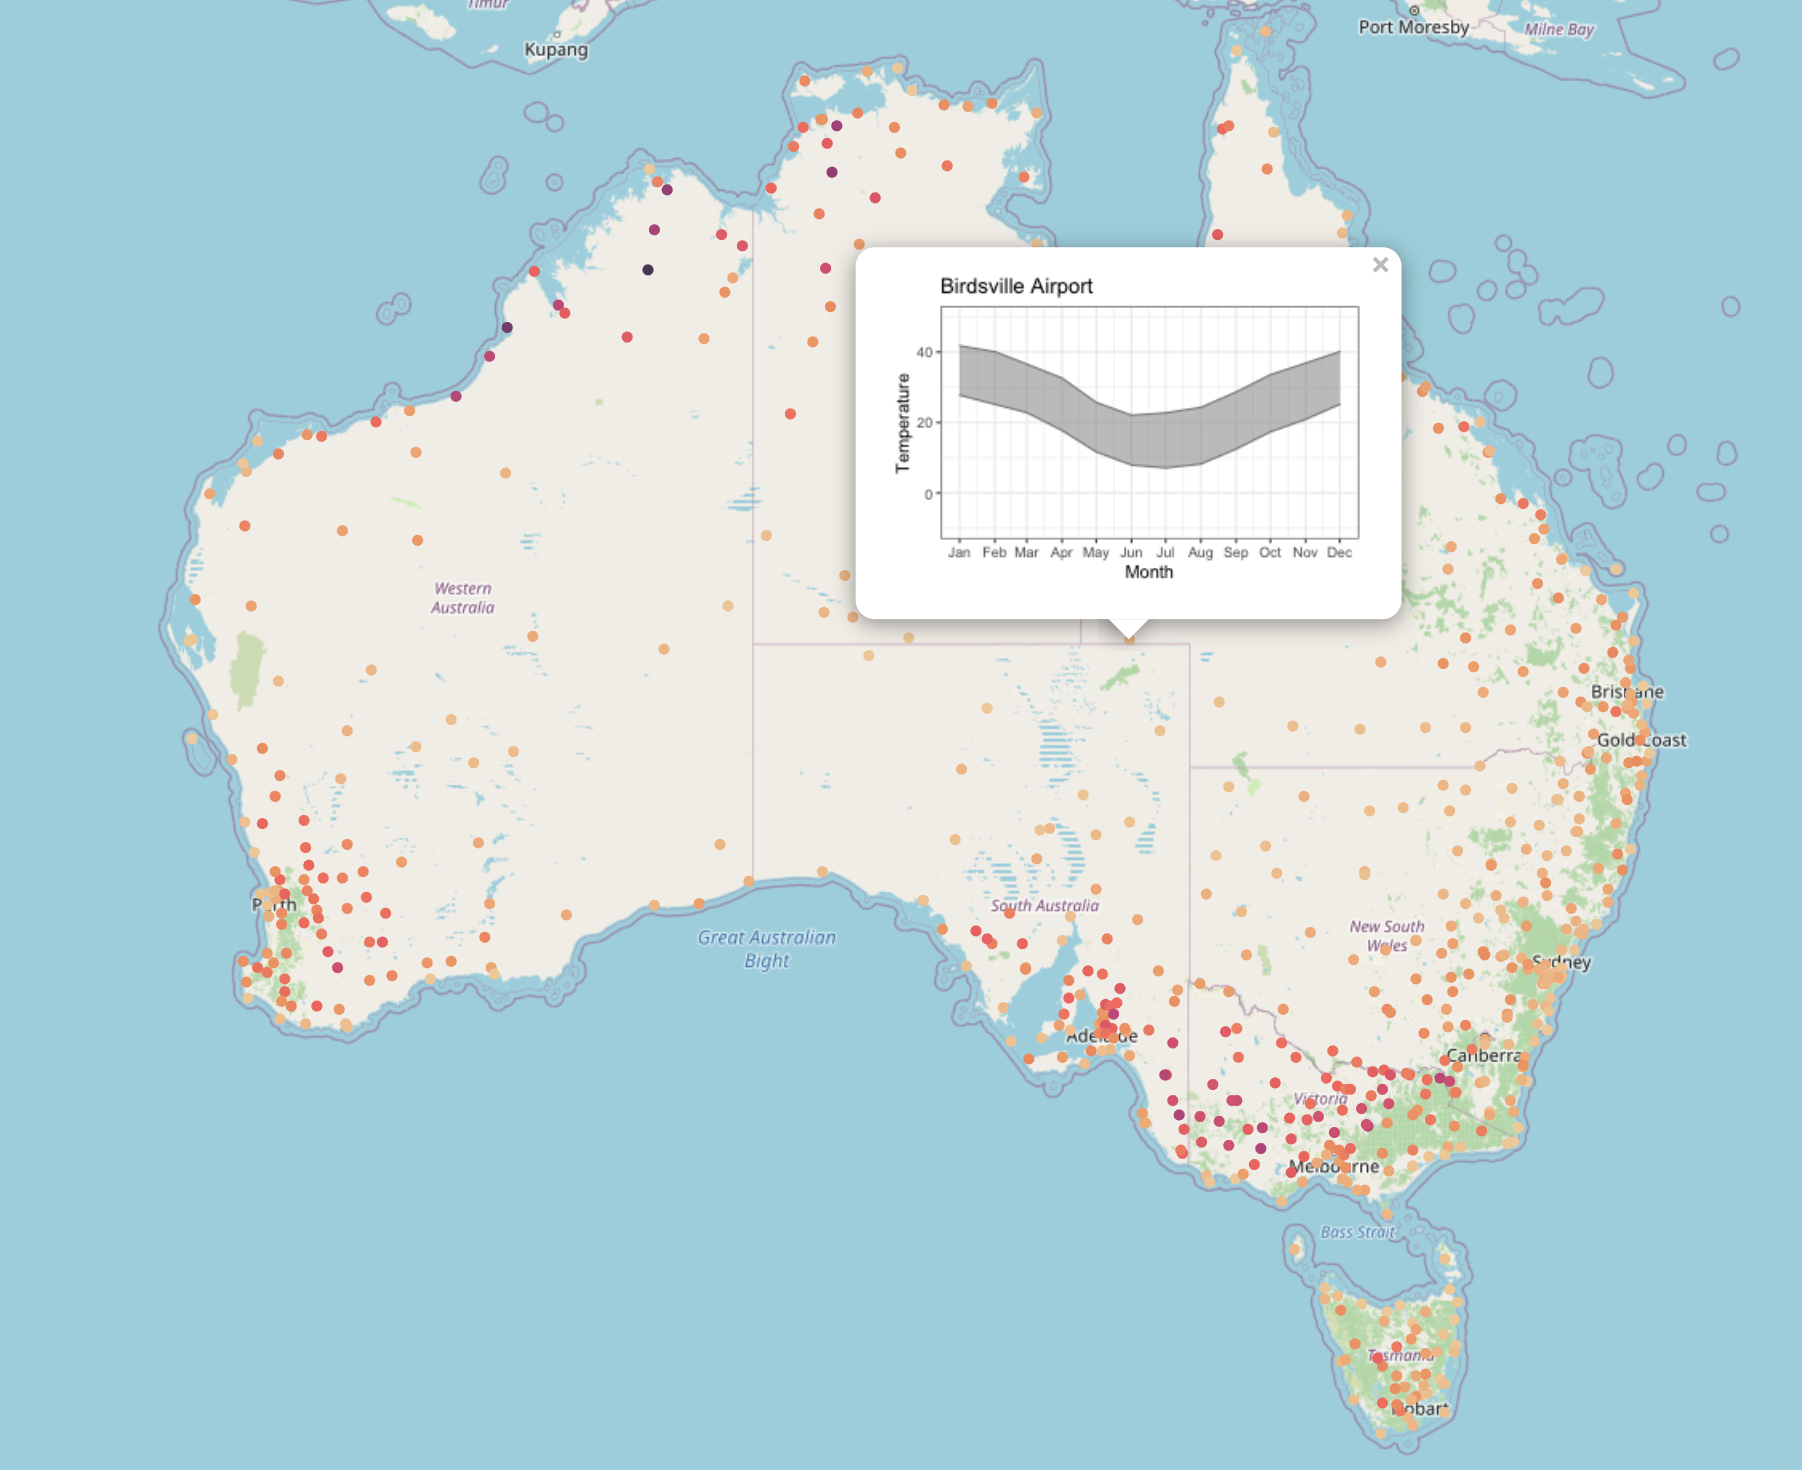
\includegraphics[width=0.45\linewidth,height=0.25\textheight]{/Users/sherryzhang/Documents/research/paper-cubble/figures/popup-mid} 

}

\caption[Screenshots of variance of monthly temperature range from 2016 to 2020 in Australia]{Screenshots of variance of monthly temperature range from 2016 to 2020 in Australia. Upon clicking a single station on the leaftlet up, the temperature band will be shown as a subplot in the popup box.}\label{fig:interactive-popup}
\end{figure}
\end{CodeChunk}

\hypertarget{conclusion}{%
\section{Conclusion}\label{conclusion}}

This paper describes the \proglang{R} package \texttt{cubble} for
manipulating and visualising spatio-temporal data. A new data structure,
that builds from the \texttt{rowwise\_df} and \texttt{grouped\_df} class
in the tidyverse ecosystem, is proposed to connect the spatial and
temporal variables in the spatio-temporal data. This design frees the
data analysts from spending time on organising variables of different
observational units. The data structure is also flexible to the
techniques and packages analysts use to analyse the data, for example,
in the matching example in section 4.3, users are free to use algorithms
from another pacakge to cluster stations. Further development and
maintenance of the package involves responding to changes in the
tidyverse packages that \texttt{cubble} imports, in particular,
\texttt{tibble}, \texttt{tidyr}, and \texttt{dplyr}. Another area for
further development is to extend \texttt{cubble} to other spatial
objects other than points.

\hypertarget{acknowledgement}{%
\section{Acknowledgement}\label{acknowledgement}}

This work is funded by the Commonwealth Scientific and Industrial
Research Organisation (CSIRO) Data61 Scholarship and started while
Nicolas Langrené was affiliated with CSIRO's Data61. The article is
created using \pkg{knitr} \citep{knitr} and \pkg{rmarkdown}
\citep{rmarkdown} in R. The source code for reproducing this paper can
be found at: \url{https://github.com/huizezhang-sherry/paper-cubble}.

\hypertarget{appendix}{%
\section{Appendix}\label{appendix}}

\begin{CodeChunk}
\begin{figure}

{\centering 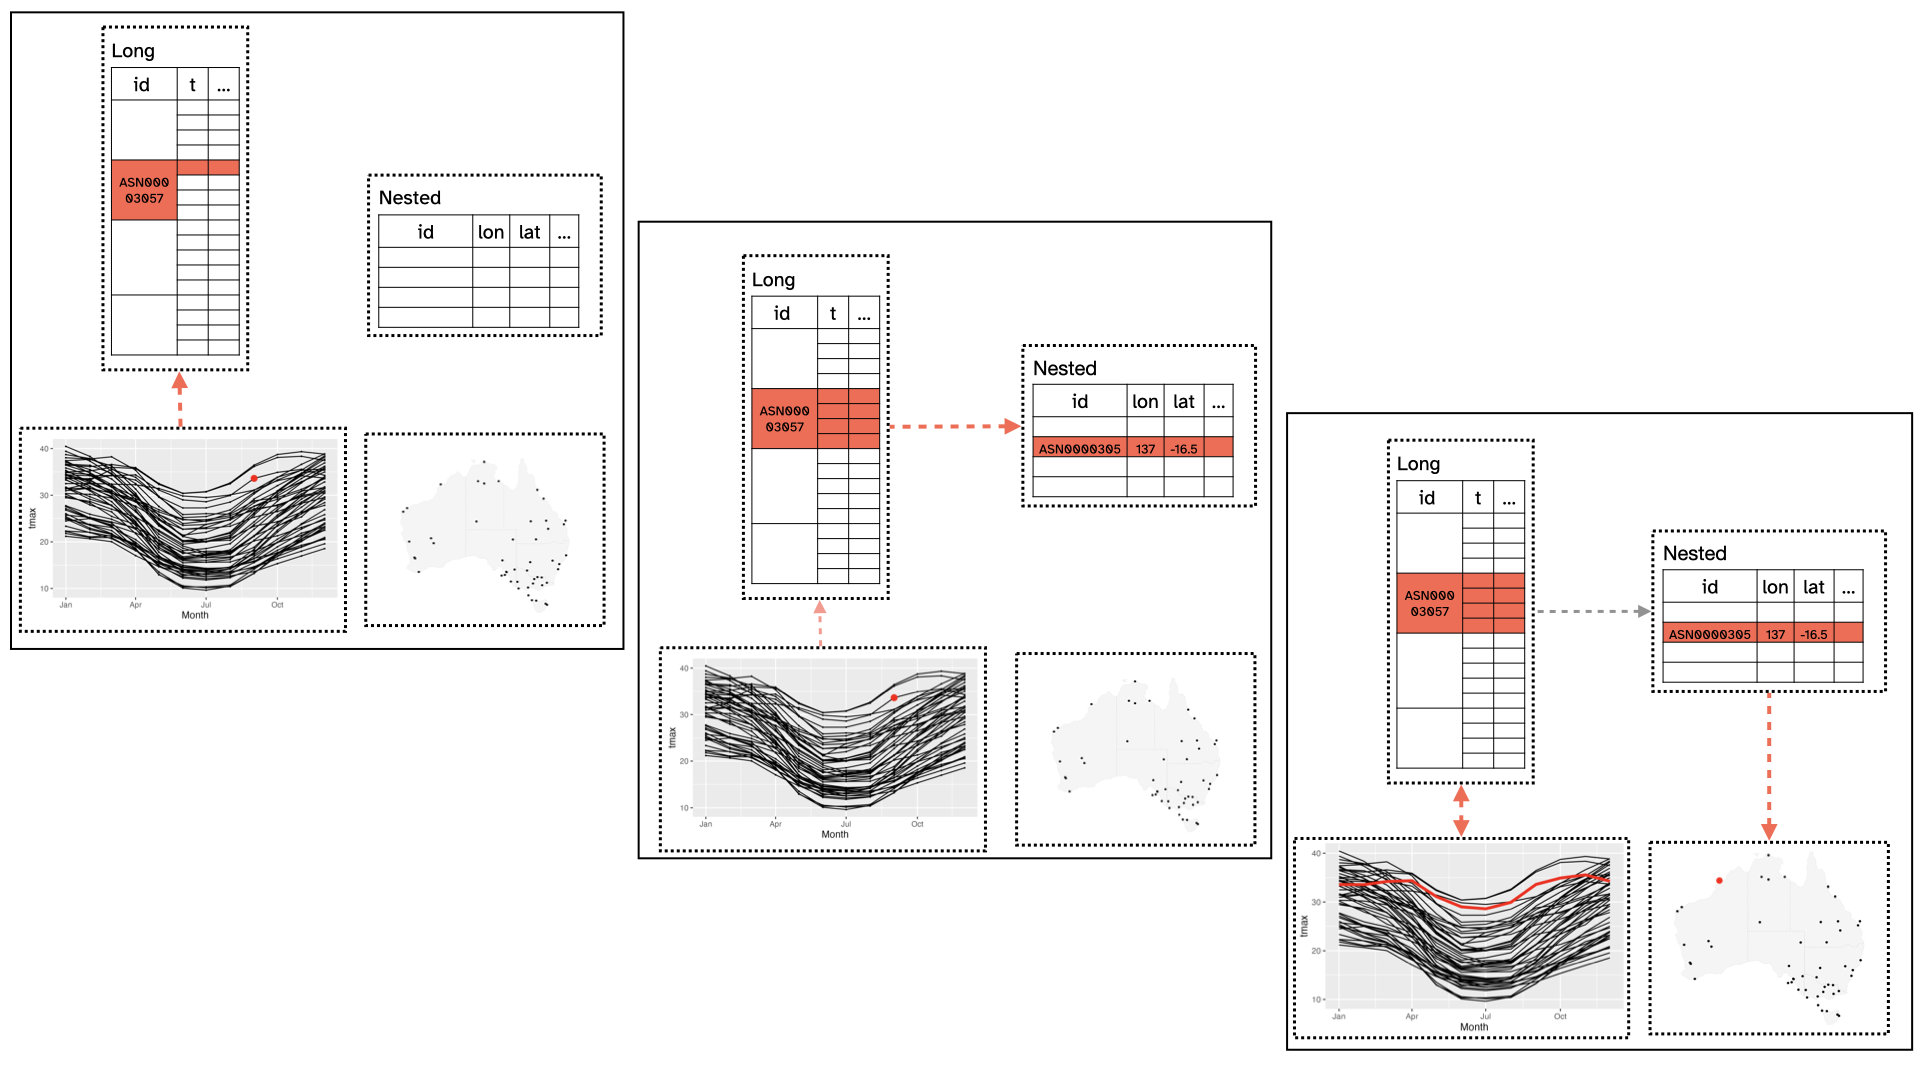
\includegraphics[width=1\linewidth,height=0.4\textheight]{/Users/sherryzhang/Documents/research/paper-cubble/figures/diagram-keynotes/diagram-keynotes.005} 

}

\caption[demon interactivity]{demon interactivity}\label{fig:illu-interactive-2}
\end{figure}
\end{CodeChunk}

\bibliography{references.bib}


\end{document}
